% Contenidos del capítulo.
% Las secciones presentadas son orientativas y no representan
% necesariamente la organización que debe tener este capítulo.

% Diagramas de clases, de secuencia, de despliegue, diseño de
% pantallas, etc

En esta sección se va a introducir el diseño o arquitectura del sistema mediante diagramas
de componentes de cada uno de los componentes lógicos que forman los subsistemas
de la aplicación. Además, se va a especificar diagramas de secuencia más precisos para
cada una de las funcionalidades de los componentes de cada subsistema. Para finalizar, se muestra un diagrama
de despliegue en el que se podrá observar los nodos a desplegar y el empaquetamiento de cada
componente.

\section{Arquitectura de componentes}

\subsection{Arquitectura de Componentes del Sistema Web}
La Figura~\ref{fig:componentes_sistema} muestra el diagrama de componentes del sistema desarrollado, el cual está estructurado en tres capas tecnológicas principales: \textbf{Frontend Web}, \textbf{Backend Principal} y \textbf{Subsistemas especializados y servicios externos}. Esta arquitectura modular permite una escalabilidad horizontal clara, así como la integración sencilla de nuevas funcionalidades.

\begin{sidewaysfigure}
    \centering
    
\includegraphics[width=0.95\textheight]{figs/arquitectura.pdf}
    \caption{Diagrama de componentes del sistema.\label{fig:componentes_sistema}}
\end{sidewaysfigure}


\subsubsection*{1. Plataforma Web Frontend}
Implementada con \texttt{Angular} y tecnologías estándar como \texttt{HTML5}, la interfaz de usuario está compuesta por varios componentes funcionales:

\begin{itemize}
\item \textbf{Login}, \textbf{Register}, \textbf{Gestor}, \textbf{Inicio}, \textbf{Reservas}, \textbf{LaCasa}, \textbf{Entorno}, \textbf{Recomendaciones}, \textbf{ComoLlegar}:
Son los componentes visuales que representan cada una de las vistas principales.

\item \textbf{Servicios asociados}: cada vista se comunica con el backend a través de servicios como:
\begin{itemize}
    \item \texttt{AuthService}: gestión de autenticación y login.
    \item \texttt{RegistroService}: registro de usuarios.
    \item \texttt{ReserveService}: gestión de reservas.
    \item \texttt{WeatherService}: consulta de clima.
    \item \texttt{ContactoService}: envío de formularios de contacto.
    \item \texttt{ReviewService}: envío y recuperación de reseñas.
    \item \texttt{MediaService}: carga de publicaciones desde redes sociales.
    \item \texttt{EntornoService}: obtención de datos de recursos turísticos.
\end{itemize}
\end{itemize}

\subsubsection*{2. Sistema Principal Backend}
Este bloque implementa la lógica de negocio central mediante \texttt{Spring Boot}, \texttt{Spring WebFlux}, \texttt{Spring Security} y \texttt{Spring Data Reactive}. Sus componentes son:

\begin{itemize}
\item \textbf{Gestión de Reservas}: permite crear, actualizar y cancelar reservas, accediendo a la base de datos \texttt{PostgreSQL} mediante \texttt{R2DBC}.
\item \textbf{Seguridad y Autenticación}: implementada con \texttt{Spring Security} y \texttt{JWT}, garantiza la protección del acceso a recursos.
\item \textbf{Formulario de Contacto}: usa \texttt{JavaMailSender} para el envío de mensajes desde la web.
\item \textbf{Gestión de Reseñas}: permite a los usuarios enviar valoraciones sobre su experiencia.
\end{itemize}

Además, toda la persistencia en el sistema principal está delegada en la \textbf{base de datos SQL PostgreSQL}, que incluye las tablas \texttt{reservas}, \texttt{users/roles} y \texttt{reviews}.

\subsubsection*{3. Subsistemas especializados}
Los microservicios siguientes se encargan de tareas específicas, todos desarrollados con \texttt{Spring Boot} y tecnologías reactivas:

\begin{itemize}
\item \textbf{Subsistema de Publicaciones}:
\begin{itemize}
\item Conecta con la \textbf{API de Instagram Graph} para importar publicaciones según hashtags.
\item Almacena los datos en la colección \texttt{media} de \texttt{MongoDB}.
\end{itemize}

\item \textbf{Subsistema de Clima}:
\begin{itemize}
    \item Obtiene predicciones meteorológicas usando \textbf{Open Meteo API}.
    \item Los datos se almacenan en la colección \texttt{weatherData} en \texttt{MongoDB}.
\end{itemize}

\item \textbf{Subsistema de Recursos Municipales}:
\begin{itemize}
    \item Utiliza \texttt{JSoup} para extraer información desde \textbf{webs municipales y turísticas}.
    \item Almacena los resultados en la colección \texttt{recursos} en \texttt{MongoDB}.
\end{itemize}
\end{itemize}

\subsubsection*{4. Integraciones Externas}
\begin{itemize}
\item \textbf{Bases de datos NoSQL}: gestionadas con \texttt{MongoDB}, organizadas en colecciones específicas para medios, clima y entorno.
\item \textbf{APIs externas}: el sistema accede a fuentes de datos abiertas como \textbf{Instagram Graph API} y \textbf{Open Meteo API}.
\item \textbf{Recursos Web}: portales oficiales de entidades como \textit{Turisme Comunitat Valenciana} y \textit{Diputació de València}.
\end{itemize}


\section{Sistema principal}
En el sistema principal, el componente de reservas gestiona el flujo completo asociado a la realización y gestión de reservas por parte de los usuarios y del gestor. A continuación, se describen los diferentes procesos soportados, ilustrados mediante diagramas de secuencia.

\begin{itemize}

\item En la Figura~\ref{fig:secuencia_reserva_confirmacion}, se presenta el proceso de \textbf{confirmación de reserva}. Un \texttt{Usuario} envía una solicitud con los datos necesarios para registrar una reserva. El controlador valida los datos y consulta si el usuario existe en la base de datos. Tras almacenar la reserva en el repositorio, se envía un correo de confirmación mediante el servicio de correo electrónico. El sistema responde con un código \texttt{201 CREATED}.

\item La Figura~\ref{fig:secuencia_reserva_obtener} describe la \textbf{consulta de reservas por parte del gestor}. El \texttt{Gestor} solicita todas las reservas ordenadas por fecha de inicio. La lógica del servicio consulta el repositorio y retorna un \texttt{Flux\<Reserva\>} con los resultados.

\item En la Figura~\ref{fig:secuencia_reserva_proximas}, se representa el proceso de \textbf{obtención de reservas próximas}. En este caso, cualquier \texttt{Usuario} puede consultar las reservas a partir de la fecha actual. El sistema devuelve un \texttt{Flux\<Tuple2\<LocalDate, LocalDate\>} con los intervalos de fechas de las reservas, para que se visualicen los dias reservados en el calendario por otros usuarios.

\item La Figura~\ref{fig:secuencia_reserva_estado} detalla el flujo de \textbf{actualización del estado de una reserva}. El \texttt{Gestor} envía una petición para modificar el estado. Dependiendo del nuevo estado, se ejecutan acciones distintas: si se marca como \texttt{PAGADA}, se confirma el pago y se envía un correo de confirmación; si se marca como \texttt{CANCELADA}, se notifica la cancelación. En ambos casos, se actualiza la entidad y se guarda en la base de datos.

\item Por último, la Figura~\ref{fig:secuencia_reserva_usuario} ilustra la \textbf{consulta de reservas por usuario}. A través del correo electrónico, un \texttt{Usuario} puede recuperar sus reservas. El sistema filtra por email y responde con un \texttt{Flux\<Reserva\>}.

\end{itemize}


\begin{figure}[h!tb]
\centering
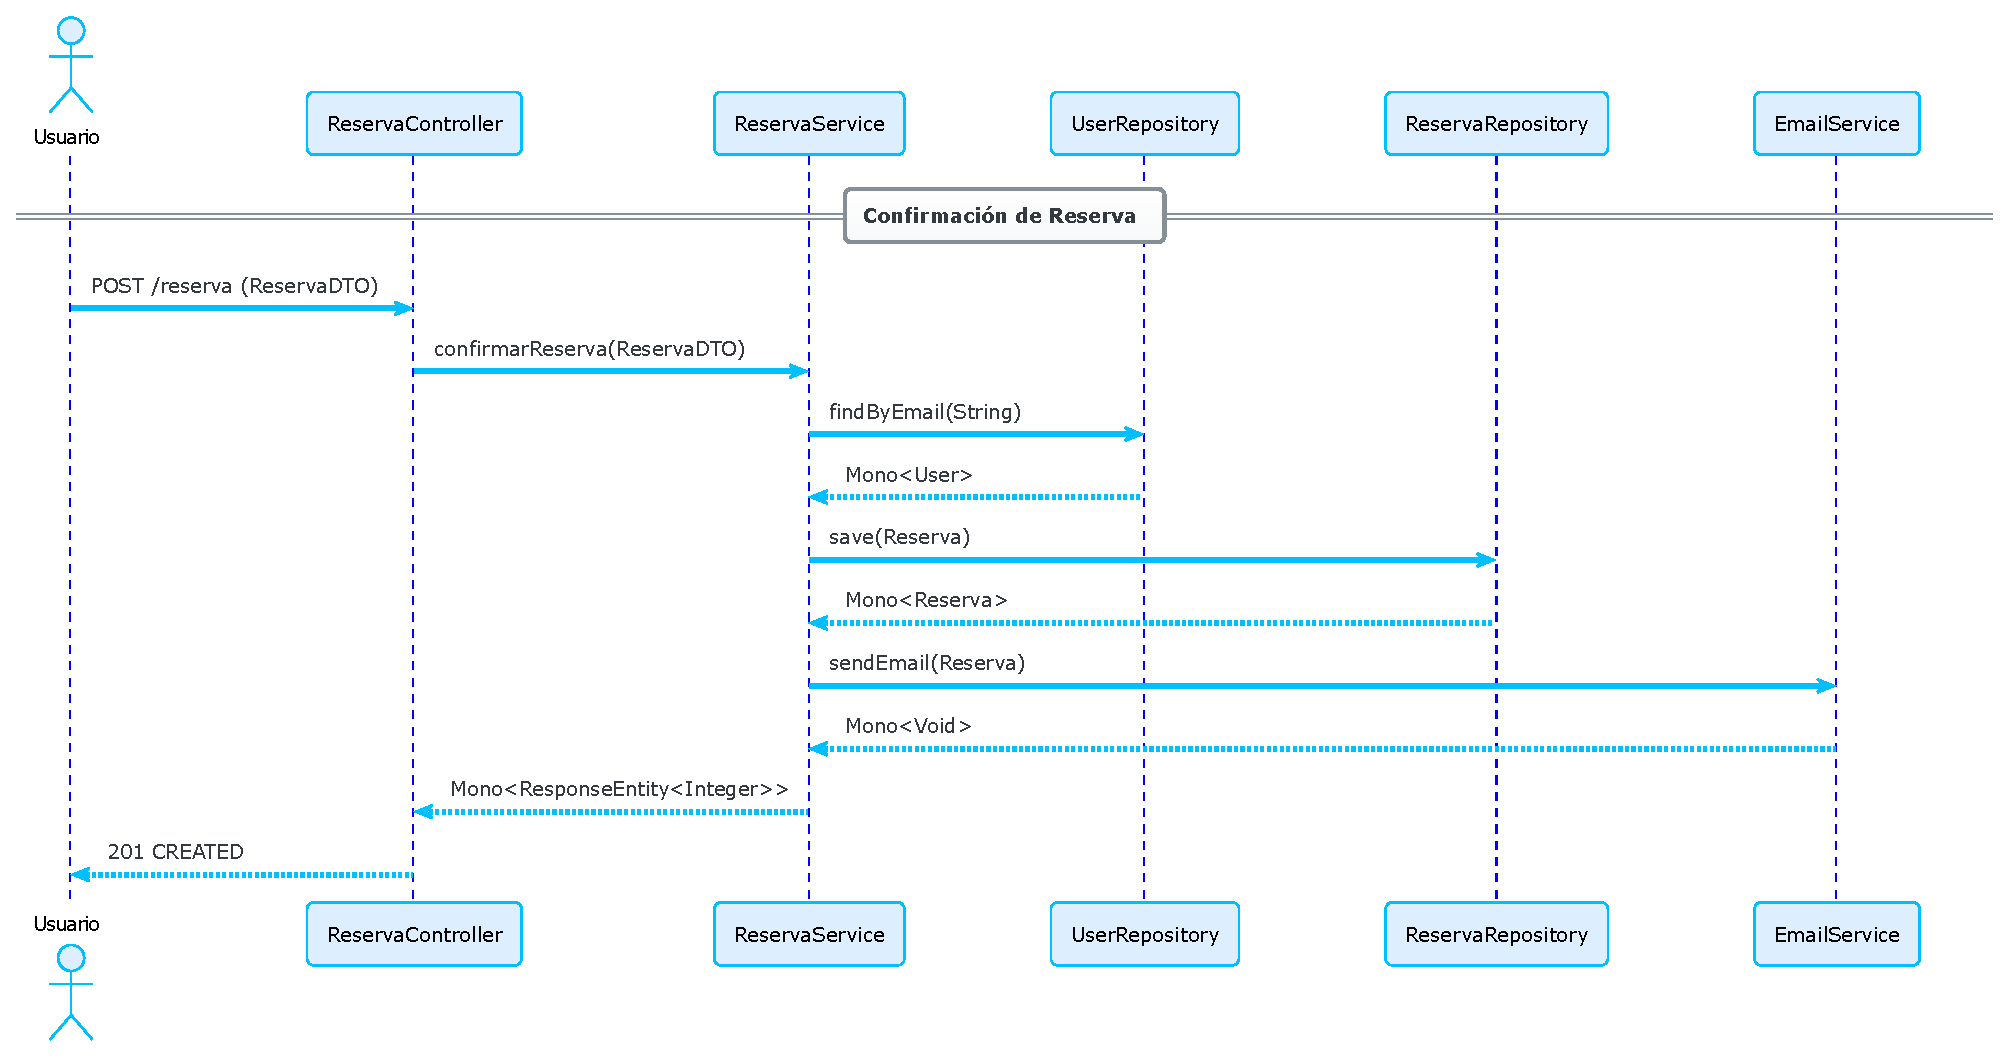
\includegraphics[width=\textwidth]{figs/secuencia_reserva_confirmacion.pdf}
\caption{Diagrama de secuencia - Confirmación de reserva.\label{fig:secuencia_reserva_confirmacion}}

\end{figure}

\begin{figure}[h!tb]
\centering
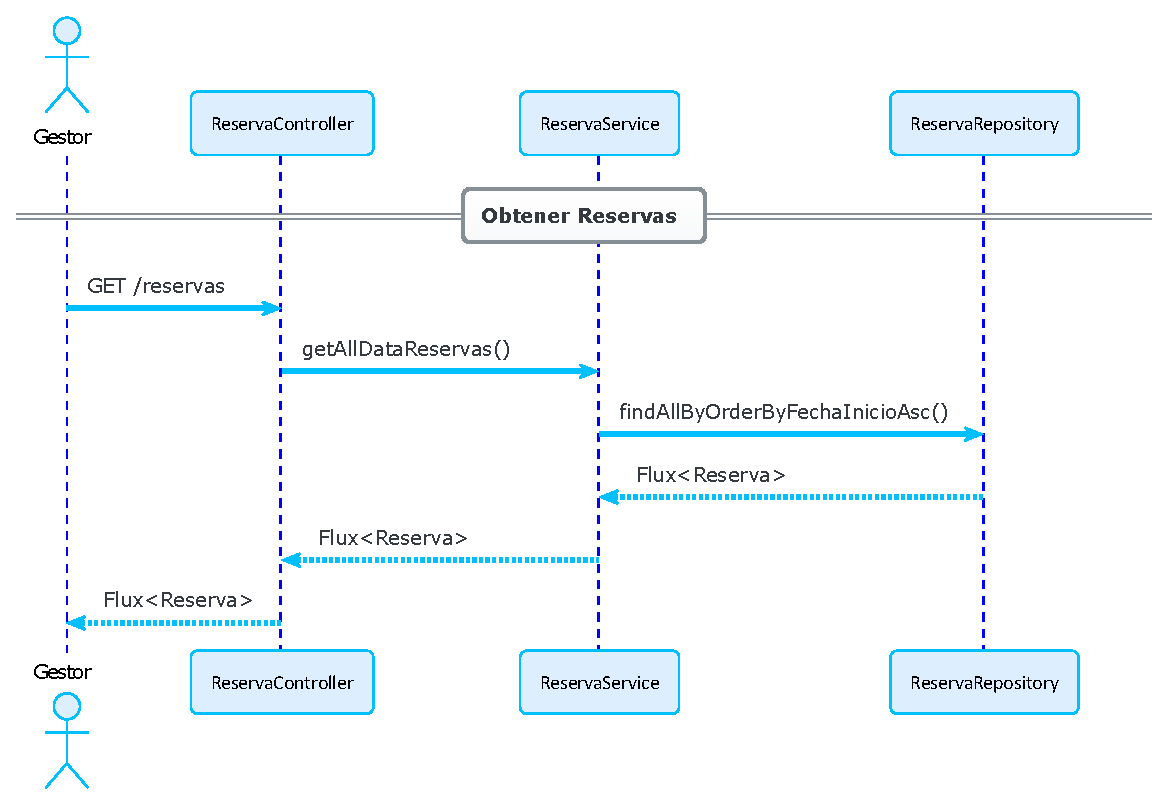
\includegraphics[width=\textwidth]{figs/secuencia_reserva_gestor_get.pdf}
\caption{Diagrama de secuencia - Obtener reservas (Gestor).\label{fig:secuencia_reserva_obtener}}
\end{figure}

\begin{figure}[h!tb]
\centering
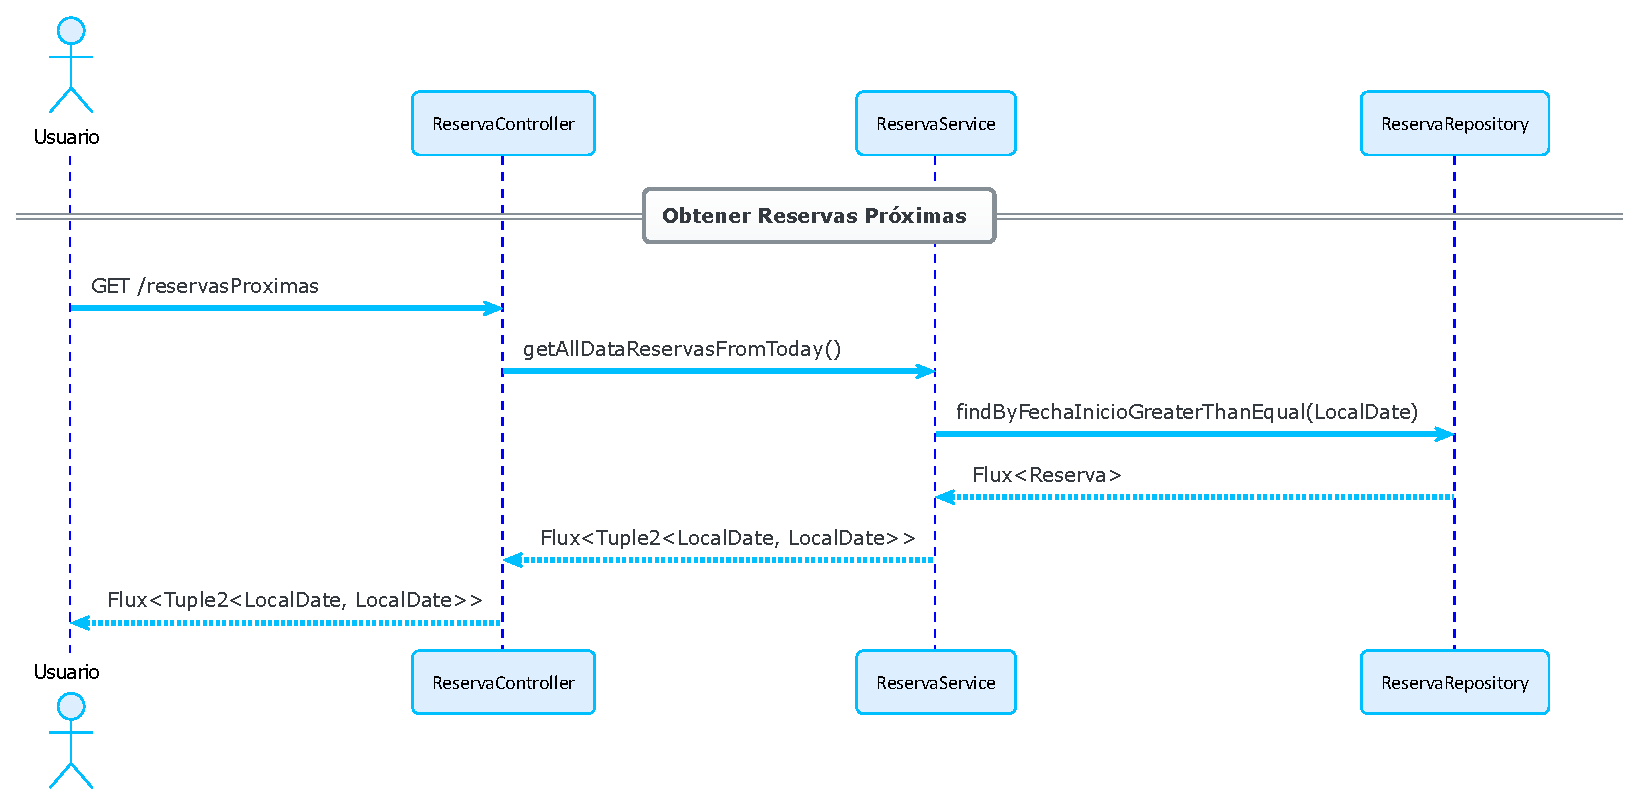
\includegraphics[width=\textwidth]{figs/secuencia_reserva_proximas.pdf}
\caption{Diagrama de secuencia - Obtener reservas próximas.\label{fig:secuencia_reserva_proximas}}
\end{figure}

\begin{figure}[h!tb]
\centering
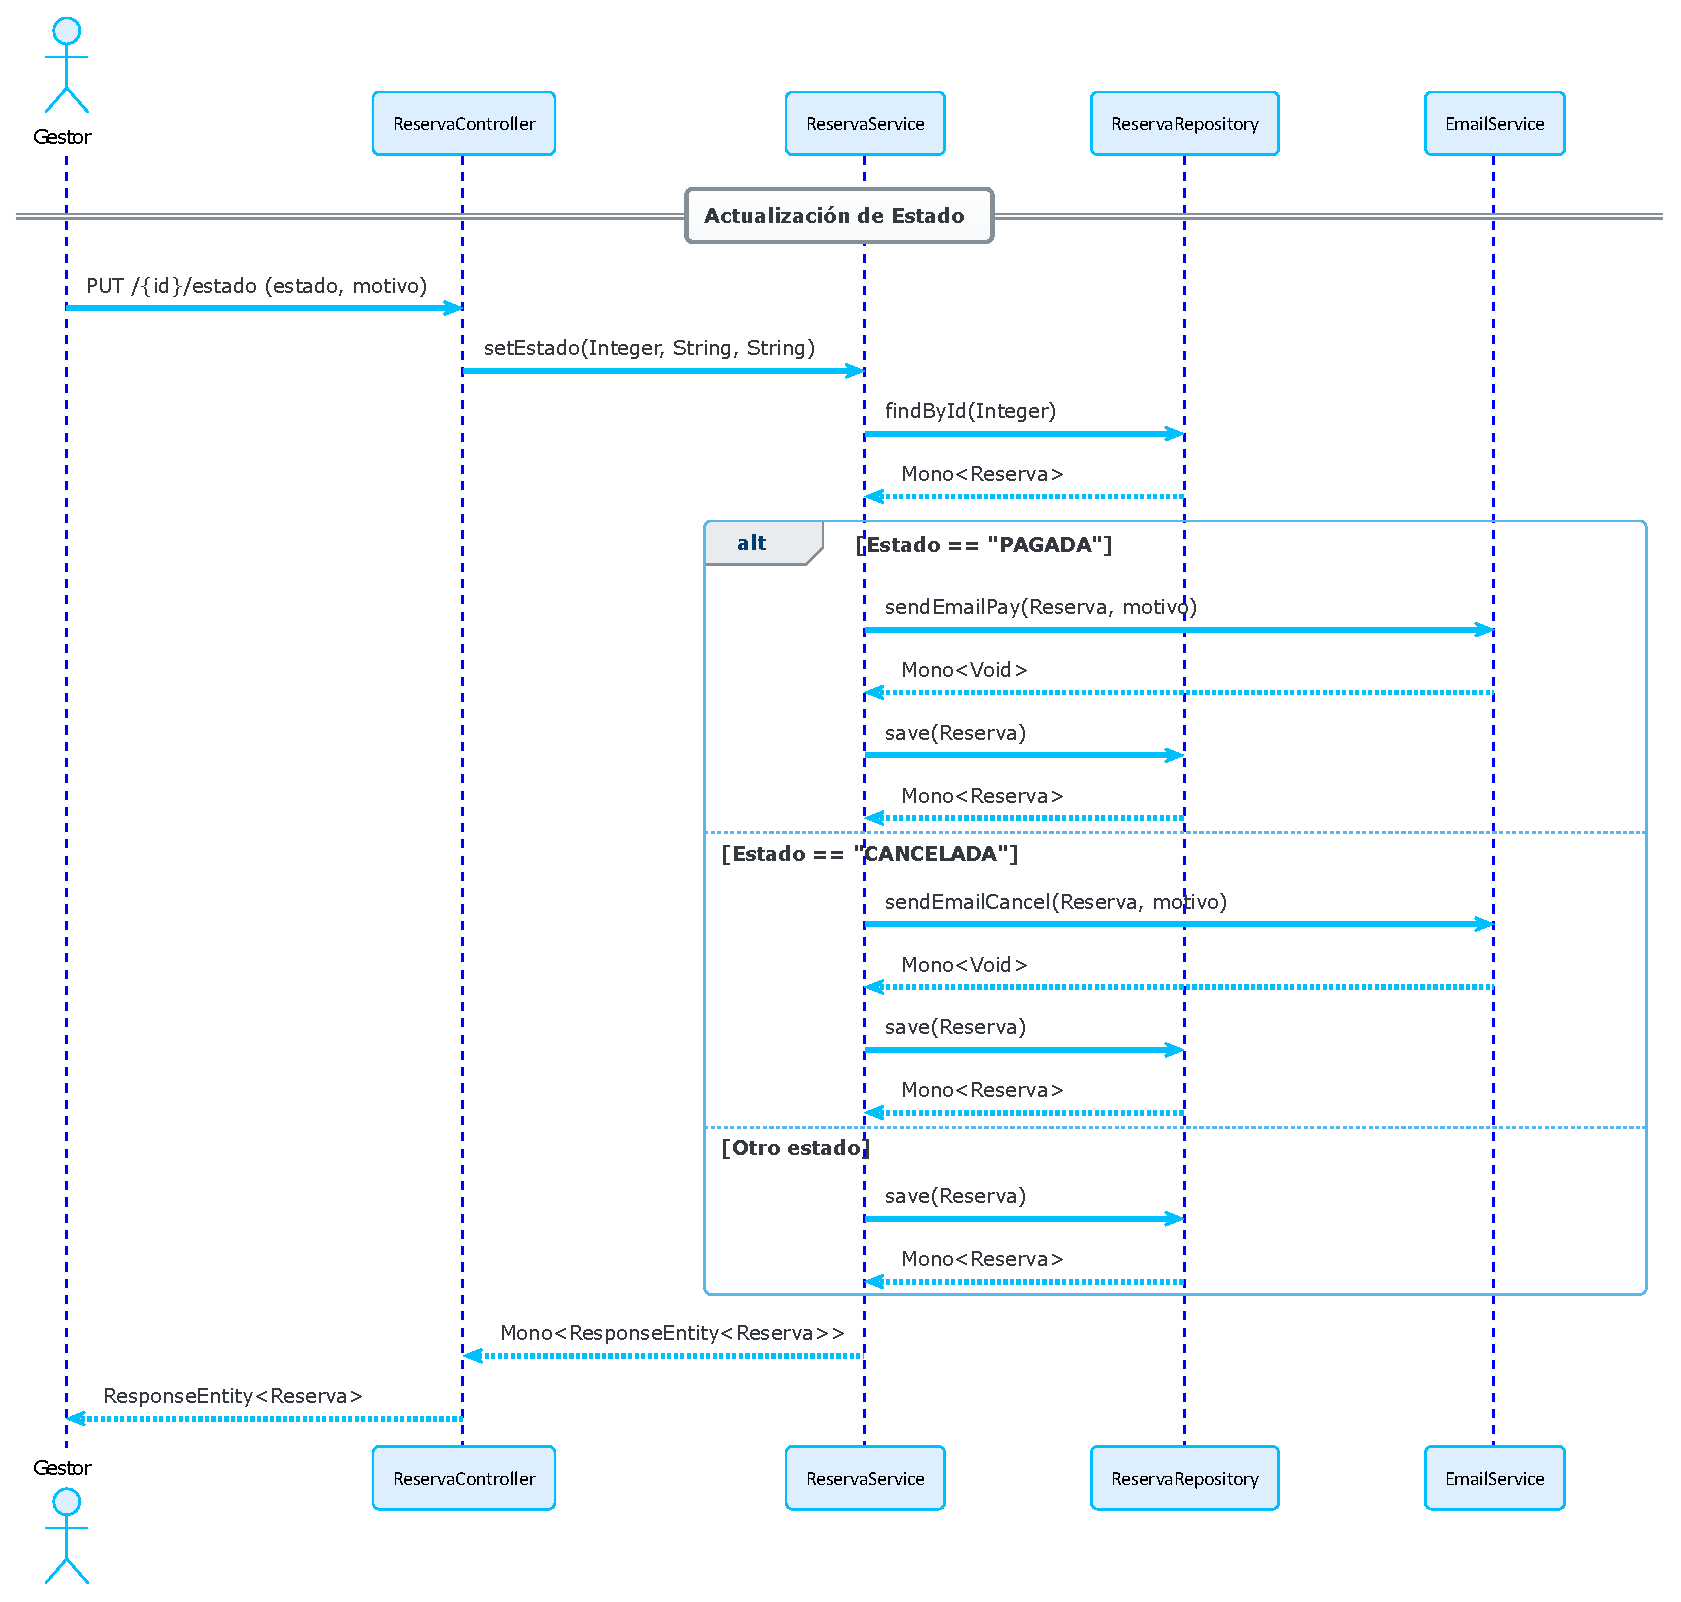
\includegraphics[width=\textwidth]{figs/secuencia_reserva_estado.pdf}
\caption{Diagrama de secuencia - Actualización de estado.\label{fig:secuencia_reserva_estado}}
\end{figure}

\begin{figure}[h!tb]
\centering
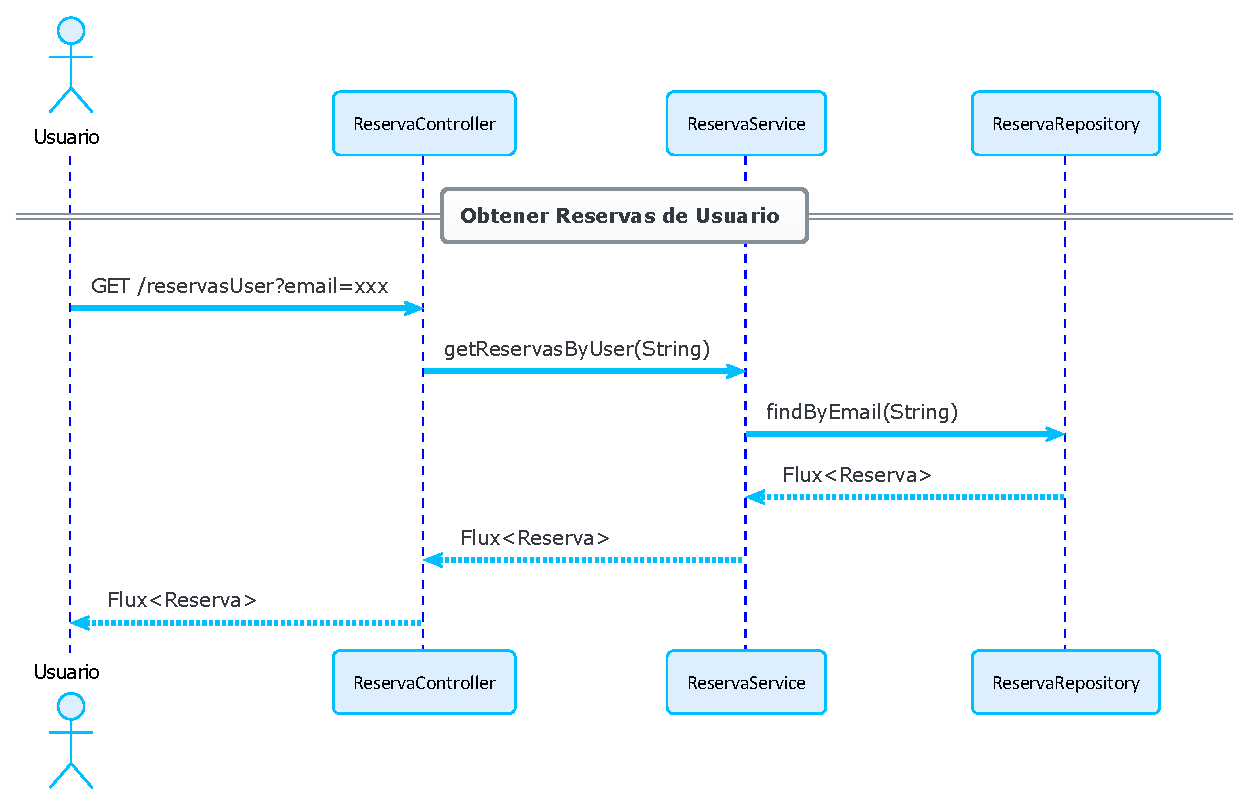
\includegraphics[width=\textwidth]{figs/secuencia_reserva_usuario.pdf}
\caption{Diagrama de secuencia - Obtener reservas por usuario.\label{fig:secuencia_reserva_usuario}}
\end{figure}
Después, se encuentra el componente de gestión de reseñas. En este módulo, los usuarios que hayan realizado una reserva (rol \texttt{CLIENTE}) podrán dejar reseñas en la aplicación, las cuales podrán ser consultadas por cualquier otro usuario. Este componente se divide en dos funcionalidades principales: añadir una reseña y consultar las reseñas existentes.

En la Figura~\ref{fig:secuencia_reseña_add} se representa el flujo completo para el proceso de añadir una reseña. El usuario autenticado, con rol CLIENTE, envía una solicitud \texttt{POST} con los datos de la reseña. El controlador delega la petición al servicio, que identifica al usuario por medio del sistema de autenticación de Spring y lo inyecta en la petición. Luego, se consulta el repositorio de usuarios para recuperar la entidad correspondiente y se elimina su rol de \texttt{CLIENTE}, dado que este rol es transitorio y únicamente se asigna tras una estancia validada. Posteriormente, se guarda la reseña en el repositorio de reseñas y se devuelve una respuesta de tipo \texttt{Mono\<ResponseEntity<Review\>\>} al cliente.

\begin{figure}[h!tb]
    \centering
    \includegraphics[width=\textwidth]{figs/secuencia_reseñas_bajo.pdf}
    \caption{Diagrama de secuencia del proceso de añadir una reseña.\label{fig:secuencia_reseña_add}}
\end{figure}

En la Figura~\ref{fig:secuencia_reseña_get} se ilustra el proceso de consulta de reseñas. En este caso, cualquier usuario puede enviar una solicitud \texttt{GET} para recuperar las reseñas almacenadas. El controlador redirige la petición al servicio, que a su vez consulta el repositorio de reseñas mediante una operación reactiva que devuelve un \texttt{Flux\<Review\>} ordenado por fecha de creación en orden descendente. La respuesta se entrega finalmente al cliente en forma de una lista de reseñas disponibles.

\begin{figure}[h!tb]
    \centering
    \includegraphics[width=\textwidth]{figs/secuencia_reseñas_get.pdf}
    \caption{Diagrama de secuencia del proceso de consulta de reseñas.\label{fig:secuencia_reseña_get}}
\end{figure}
A continuación, se encuentra el componente de contacto, el cual permite a los usuarios enviar mensajes directamente al administrador de la casa rural a través de un formulario. En la Figura~\ref{fig:secuencia_contacto} se observa el diseño de la lógica de este proceso. El usuario envía una solicitud \texttt{POST} con los datos del formulario, incluyendo nombre, email y mensaje. El controlador recibe la petición y delega el envío del correo al servicio correspondiente.

El \texttt{ContactService} construye un mensaje de tipo \texttt{SimpleMailMessage} utilizando los datos proporcionados por el usuario y lo envía mediante el componente \texttt{JavaMailSender}, el cual está configurado en el sistema. Una vez enviado el correo electrónico, el servicio devuelve una respuesta de tipo \texttt{Mono\<Contact>}, que es encapsulada en un objeto \texttt{ResponseEntity} para ser devuelta al usuario con un estado HTTP 200 si todo ha ido correctamente, o 400 en caso de error.

\begin{figure}[h!tb]
    \centering
    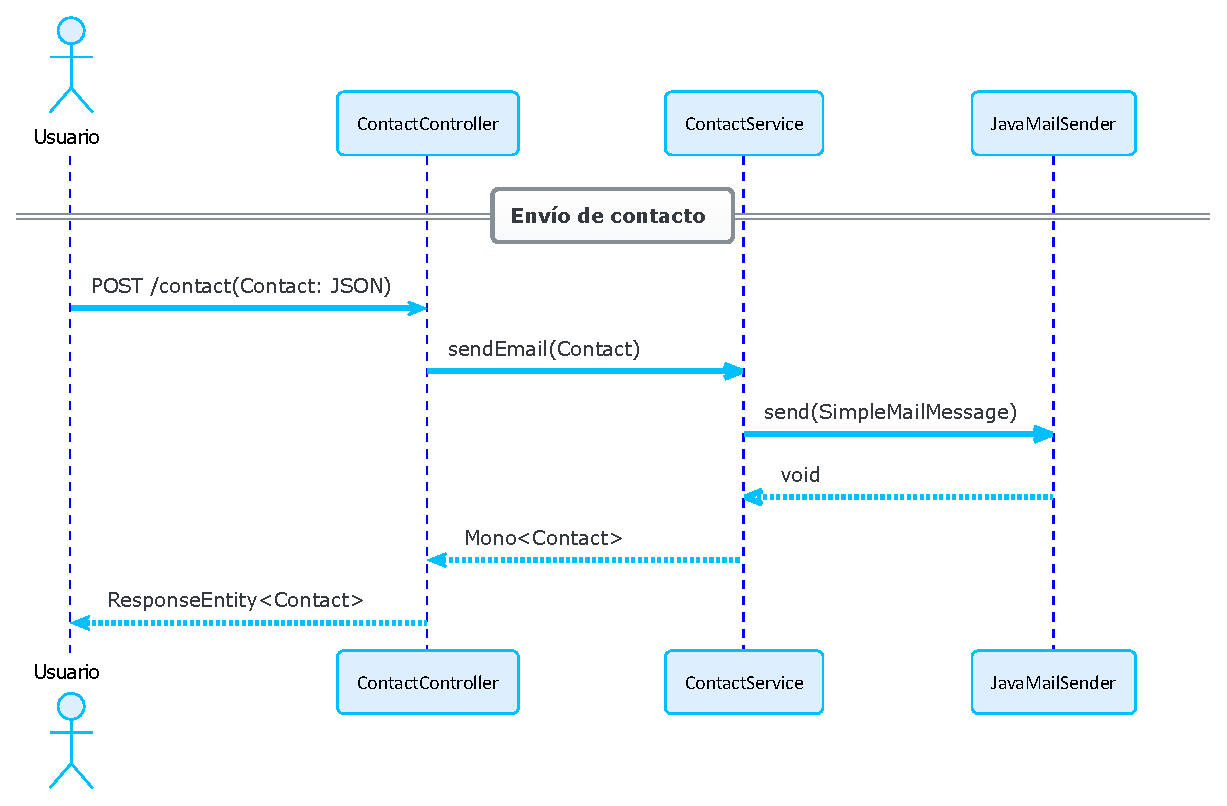
\includegraphics[width=\textwidth]{figs/secuencia_contacto.pdf}
    \caption{Diagrama de secuencia del componente de contacto.\label{fig:secuencia_contacto}}
\end{figure}

Finalmente, se encuentra el componente encargado de la seguridad el cual se especifica mediante configuración y infraestructura. Por lo tanto, se detallará en la sección de despliegue \ref{ch:despliegue} y en la implementación \ref{ch:im}
\section{Subsistema de recursos web}

En el subsistema de recursos web, uno de los componentes fundamentales es el servicio de raspado automatizado de contenidos turísticos. Este componente permite tanto a los usuarios acceder a los recursos almacenados como al sistema actualizar periódicamente la información mediante técnicas de \textit{web scraping}.

\subsection{Extracción solicitada por el usuario}

En la Figura~\ref{fig:secuencia_recursos_usuarios} se ilustra el comportamiento del sistema cuando un usuario interactúa con el \texttt{ExtraccionController} para consultar los recursos disponibles. Se representan dos casos diferenciados:

\begin{itemize}
  \item Una solicitud GET a \texttt{/api/v1/extraccion} desencadena la invocación del método \texttt{extractAllResources()} del servicio \texttt{RecursoService}, que accede a todos los documentos de la colección mediante el repositorio reactivo \texttt{RecursoRepository} y retorna un \texttt{Flux<Recurso>}.
  
  \item En el segundo caso, cuando el usuario realiza una solicitud GET a \texttt{/api/v1/extraccionFiestas}, el sistema filtra los resultados por la categoría \texttt{"fiestas"} mediante el método \texttt{findByCategoria()}.
\end{itemize}

\begin{figure}[h!tb]
    \centering
    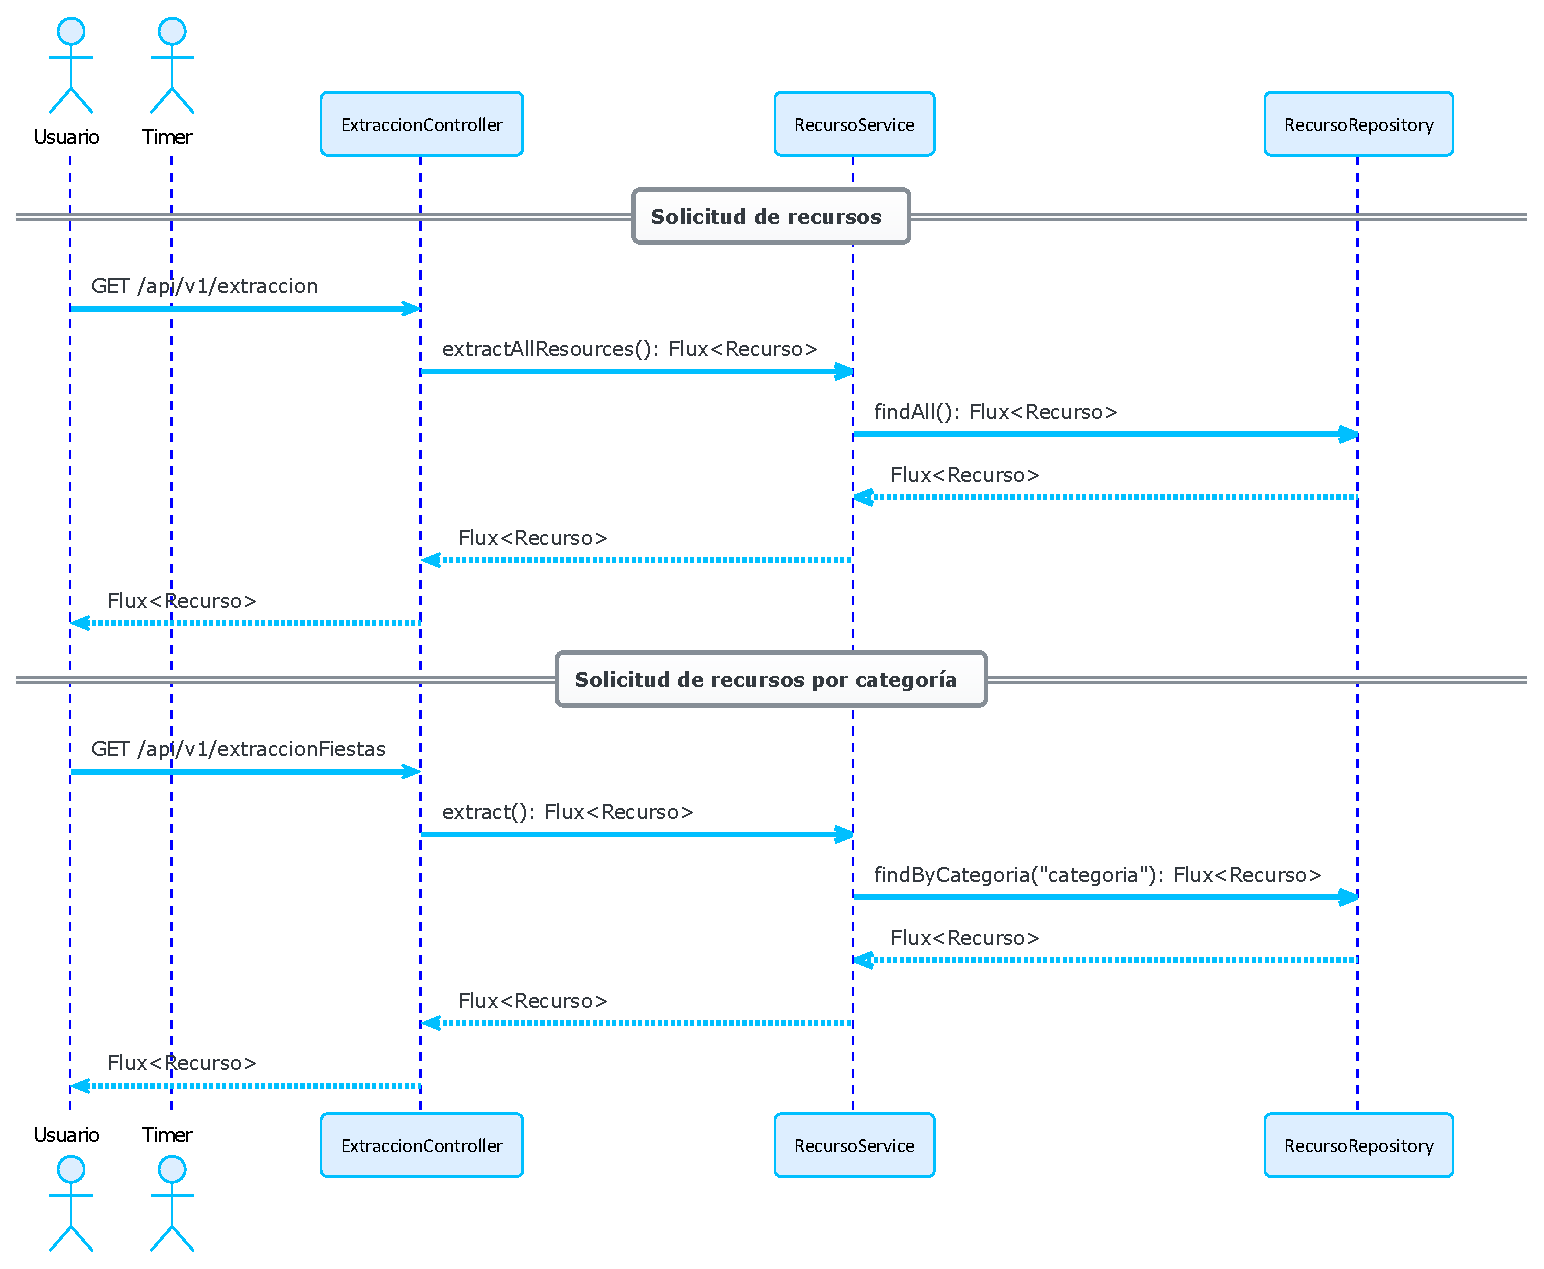
\includegraphics[width=1\textwidth]{figs/secuencia_recursos_usuarios.pdf}
    \caption{Diagrama de secuencia para solicitudes de recursos por parte de usuarios.\label{fig:secuencia_recursos_usuarios}}
\end{figure}

\subsection{Extracción programada con scraping}

En la Figura~\ref{fig:secuencia_recursos_scheduled} se representa la lógica que ejecuta la tarea de extracción programada mediante un \texttt{@Scheduled} en el servicio \texttt{RecursoService}. Esta ejecución se realiza automáticamente cada día a las 00:00 horas y tiene como objetivo extraer y almacenar información actualizada desde diversas fuentes externas.

Durante este proceso:

\begin{itemize}
  \item Se invoca secuencialmente el método \texttt{scrape()} del \texttt{ScraperService}, pasando como parámetros la URL base, el tipo de recurso (como \texttt{"monumentos"}, \texttt{"fiestas"}) y la localización (como \texttt{chelva} o \texttt{tuejar}).
  \item Internamente se llama a \texttt{ensureCollectionExists()} para asegurar que la colección \texttt{recursos} existe en MongoDB usando \texttt{ReactiveMongoTemplate}.
  \item Se realiza una conexión con cada URL mediante \textbf{JSoup} y se procesan los resultados con métodos específicos como \texttt{processChelvaMonumentosAldeas()},\\ \texttt{processTuejarPatrimonioNaturaleza()}\\ o \texttt{processTuejarFiestas()}.
  \item Cada recurso se almacena en MongoDB a través del \texttt{RecursoRepository}.
  \item Finalmente, se consulta la base de datos para verificar el estado actualizado de todos los recursos.
\end{itemize}

\begin{figure}[h!tb]
    \centering
    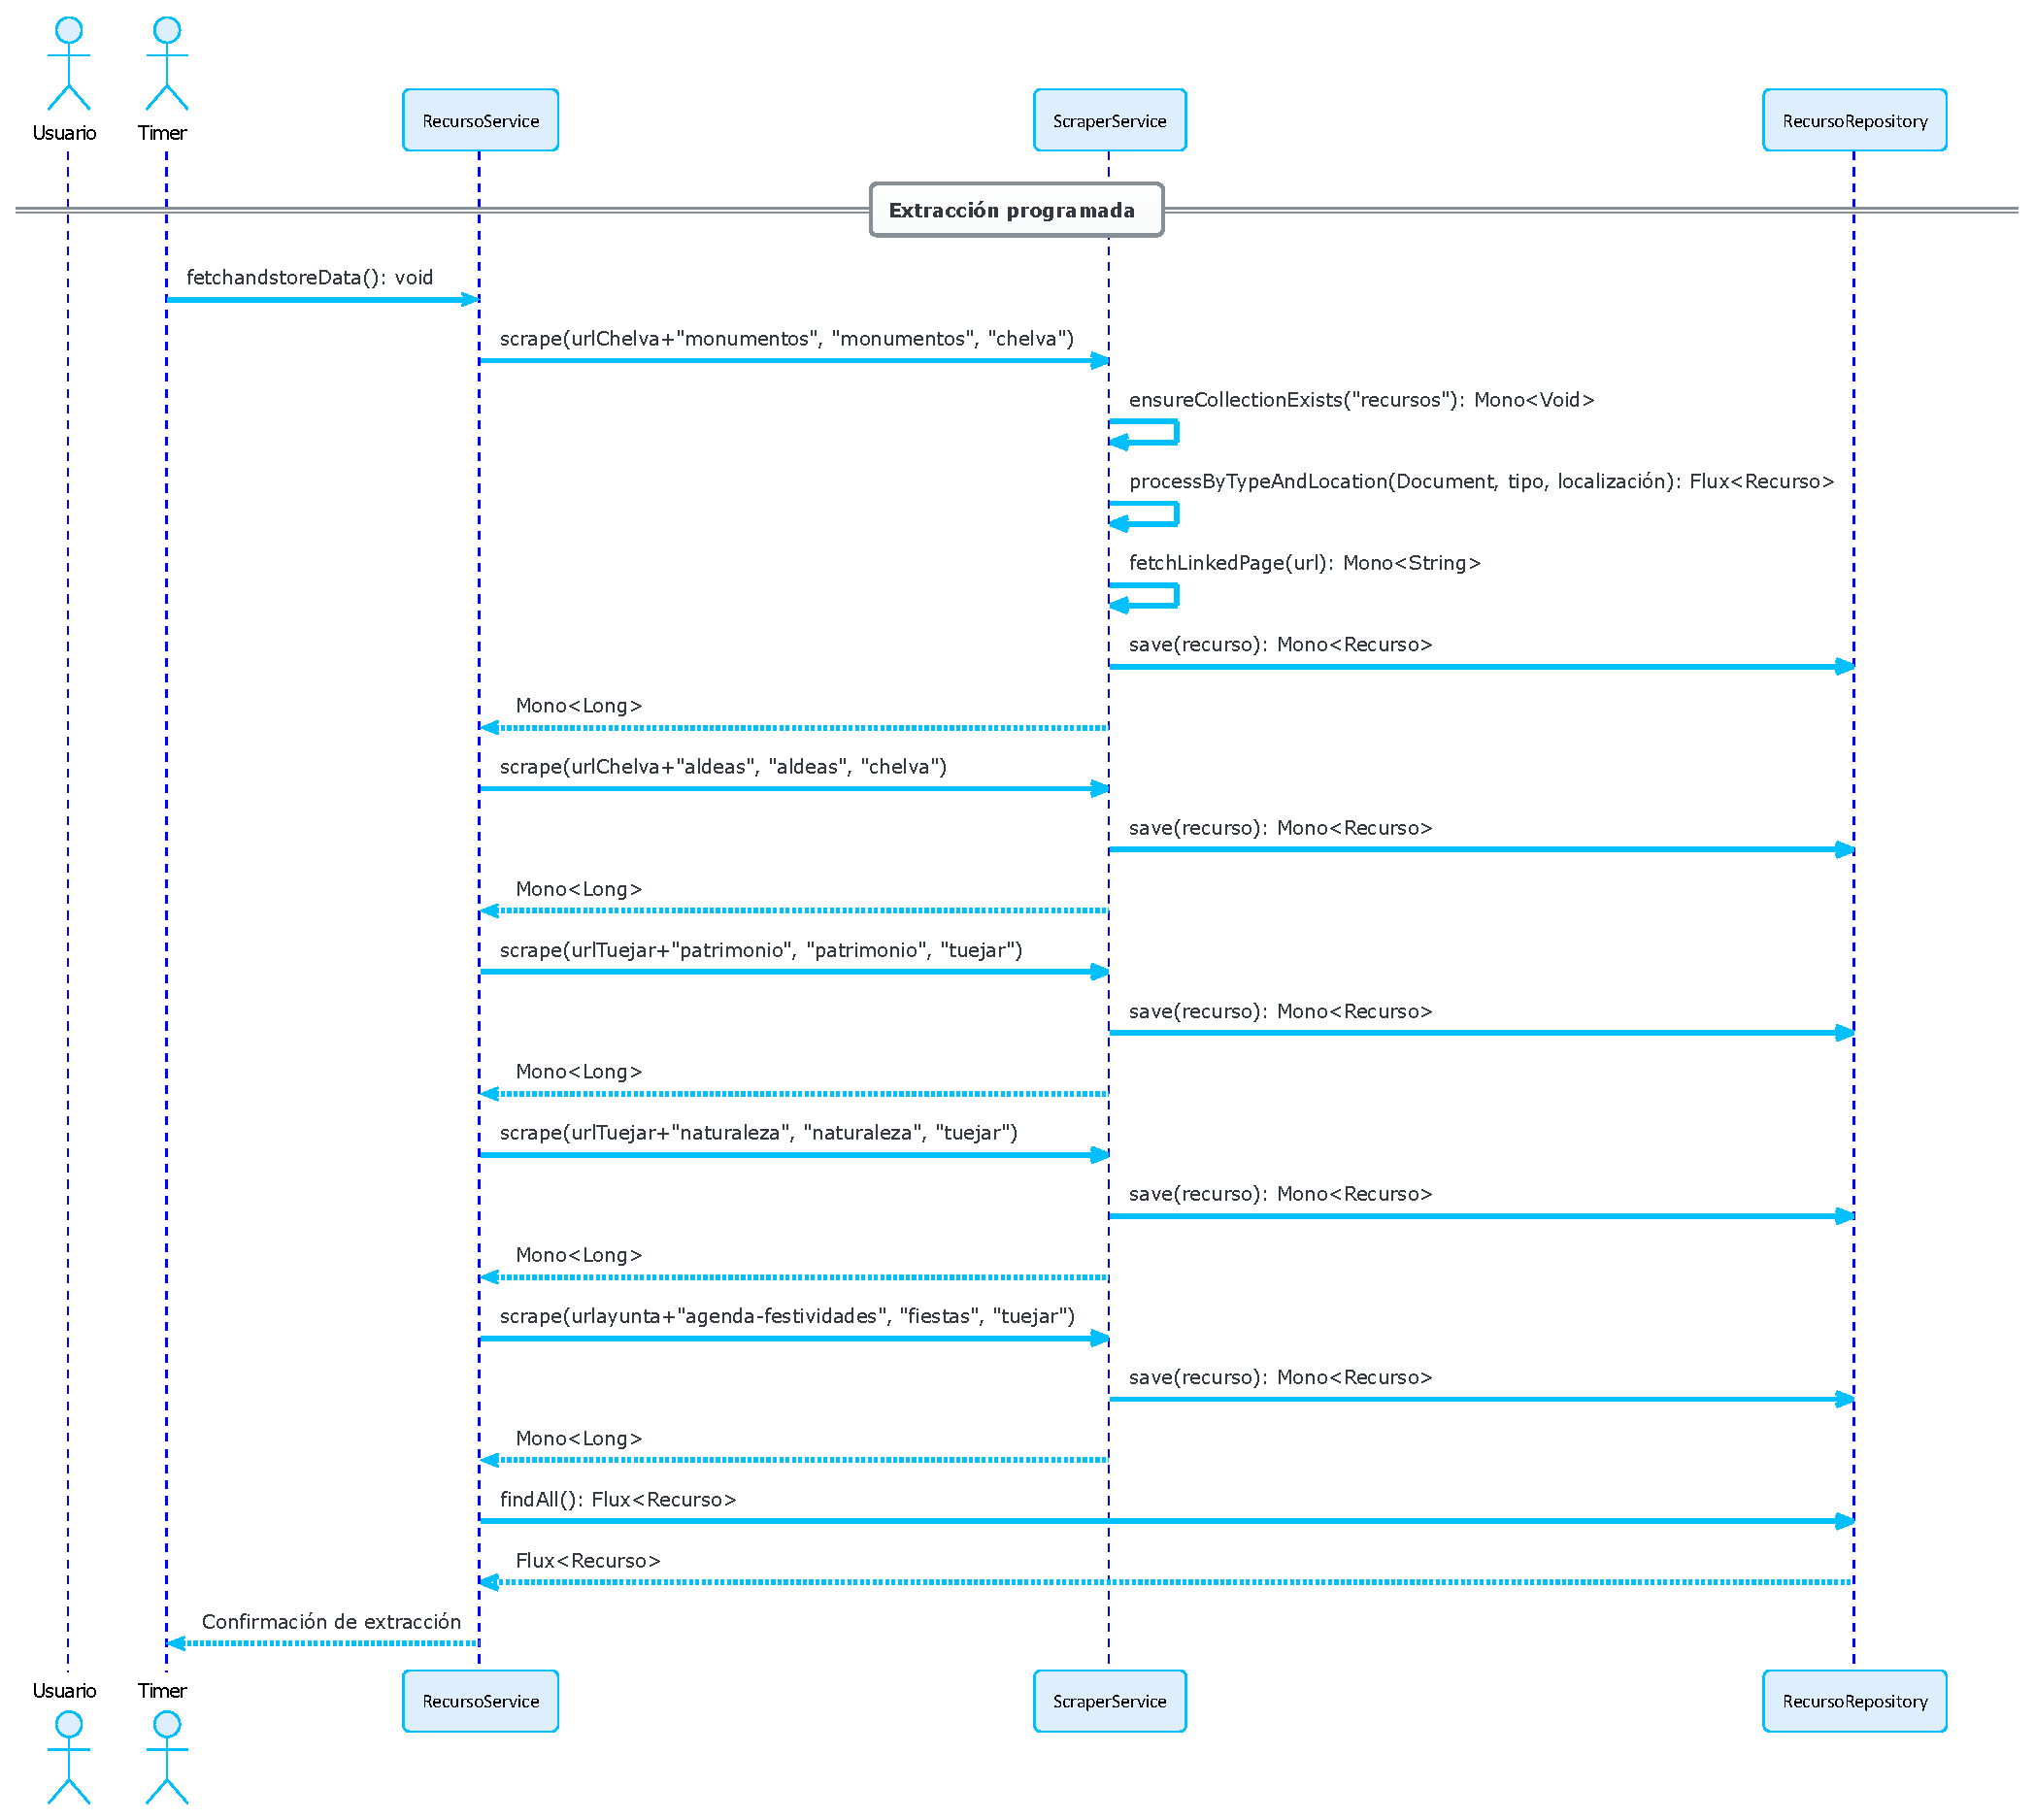
\includegraphics[width=1\textwidth]{figs/secuencia_recursos_schedule.pdf}
    \caption{Diagrama de secuencia de la extracción programada de recursos web.\label{fig:secuencia_recursos_scheduled}}
\end{figure}

\section{Subsistema de publicaciones}

En el subsistema de publicaciones el componente a especificar es el encargado de realizar la llamada a la \gls{API} de Instagram para obtener publicaciones públicas. En la Figura~\ref{fig:secuencia_publicaciones_consulta} se representa cómo interactúan los distintos elementos del sistema para gestionar consultas, así como la extracción y actualización de publicaciones desde la red social.

Cuando un \textbf{usuario} realiza una solicitud GET a \texttt{/api/v1/media}, el \texttt{MediaController} llama al \texttt{MediaService}, que busca las publicaciones en el repositorio (\texttt{MediaRepository}). Si no se encuentra ninguna entrada relevante, el servicio puede invocar la \gls{API} de Instagram a través del cliente HTTP reactivo (\texttt{WebClient}), para recuperar y actualizar los datos de forma dinámica.

Además, este proceso de sincronización se ejecuta automáticamente cada día a las 00:00 mediante un temporizador (\texttt{Timer}). El servicio obtiene el token de acceso desde el sistema de archivos mediante el \texttt{InstagramTokenService}, realiza la solicitud a la \gls{API} de Instagram y, en función de si la publicación ya existe en la base de datos o no, realiza una de las siguientes acciones:

\begin{itemize}
    \item \textbf{Guardar nueva publicación:} Si el identificador no se encuentra registrado, se almacena la nueva publicación.
    \item \textbf{Actualizar publicación existente:} Si la publicación ya existe, se actualiza su URL de medios.
\end{itemize}

Este comportamiento condicional se resume mediante una estructura \texttt{alt} que permite distinguir entre ambos flujos. El resultado del proceso se devuelve al \texttt{Timer} como indicativo de finalización.

\begin{figure}[h!tb]
    \centering
    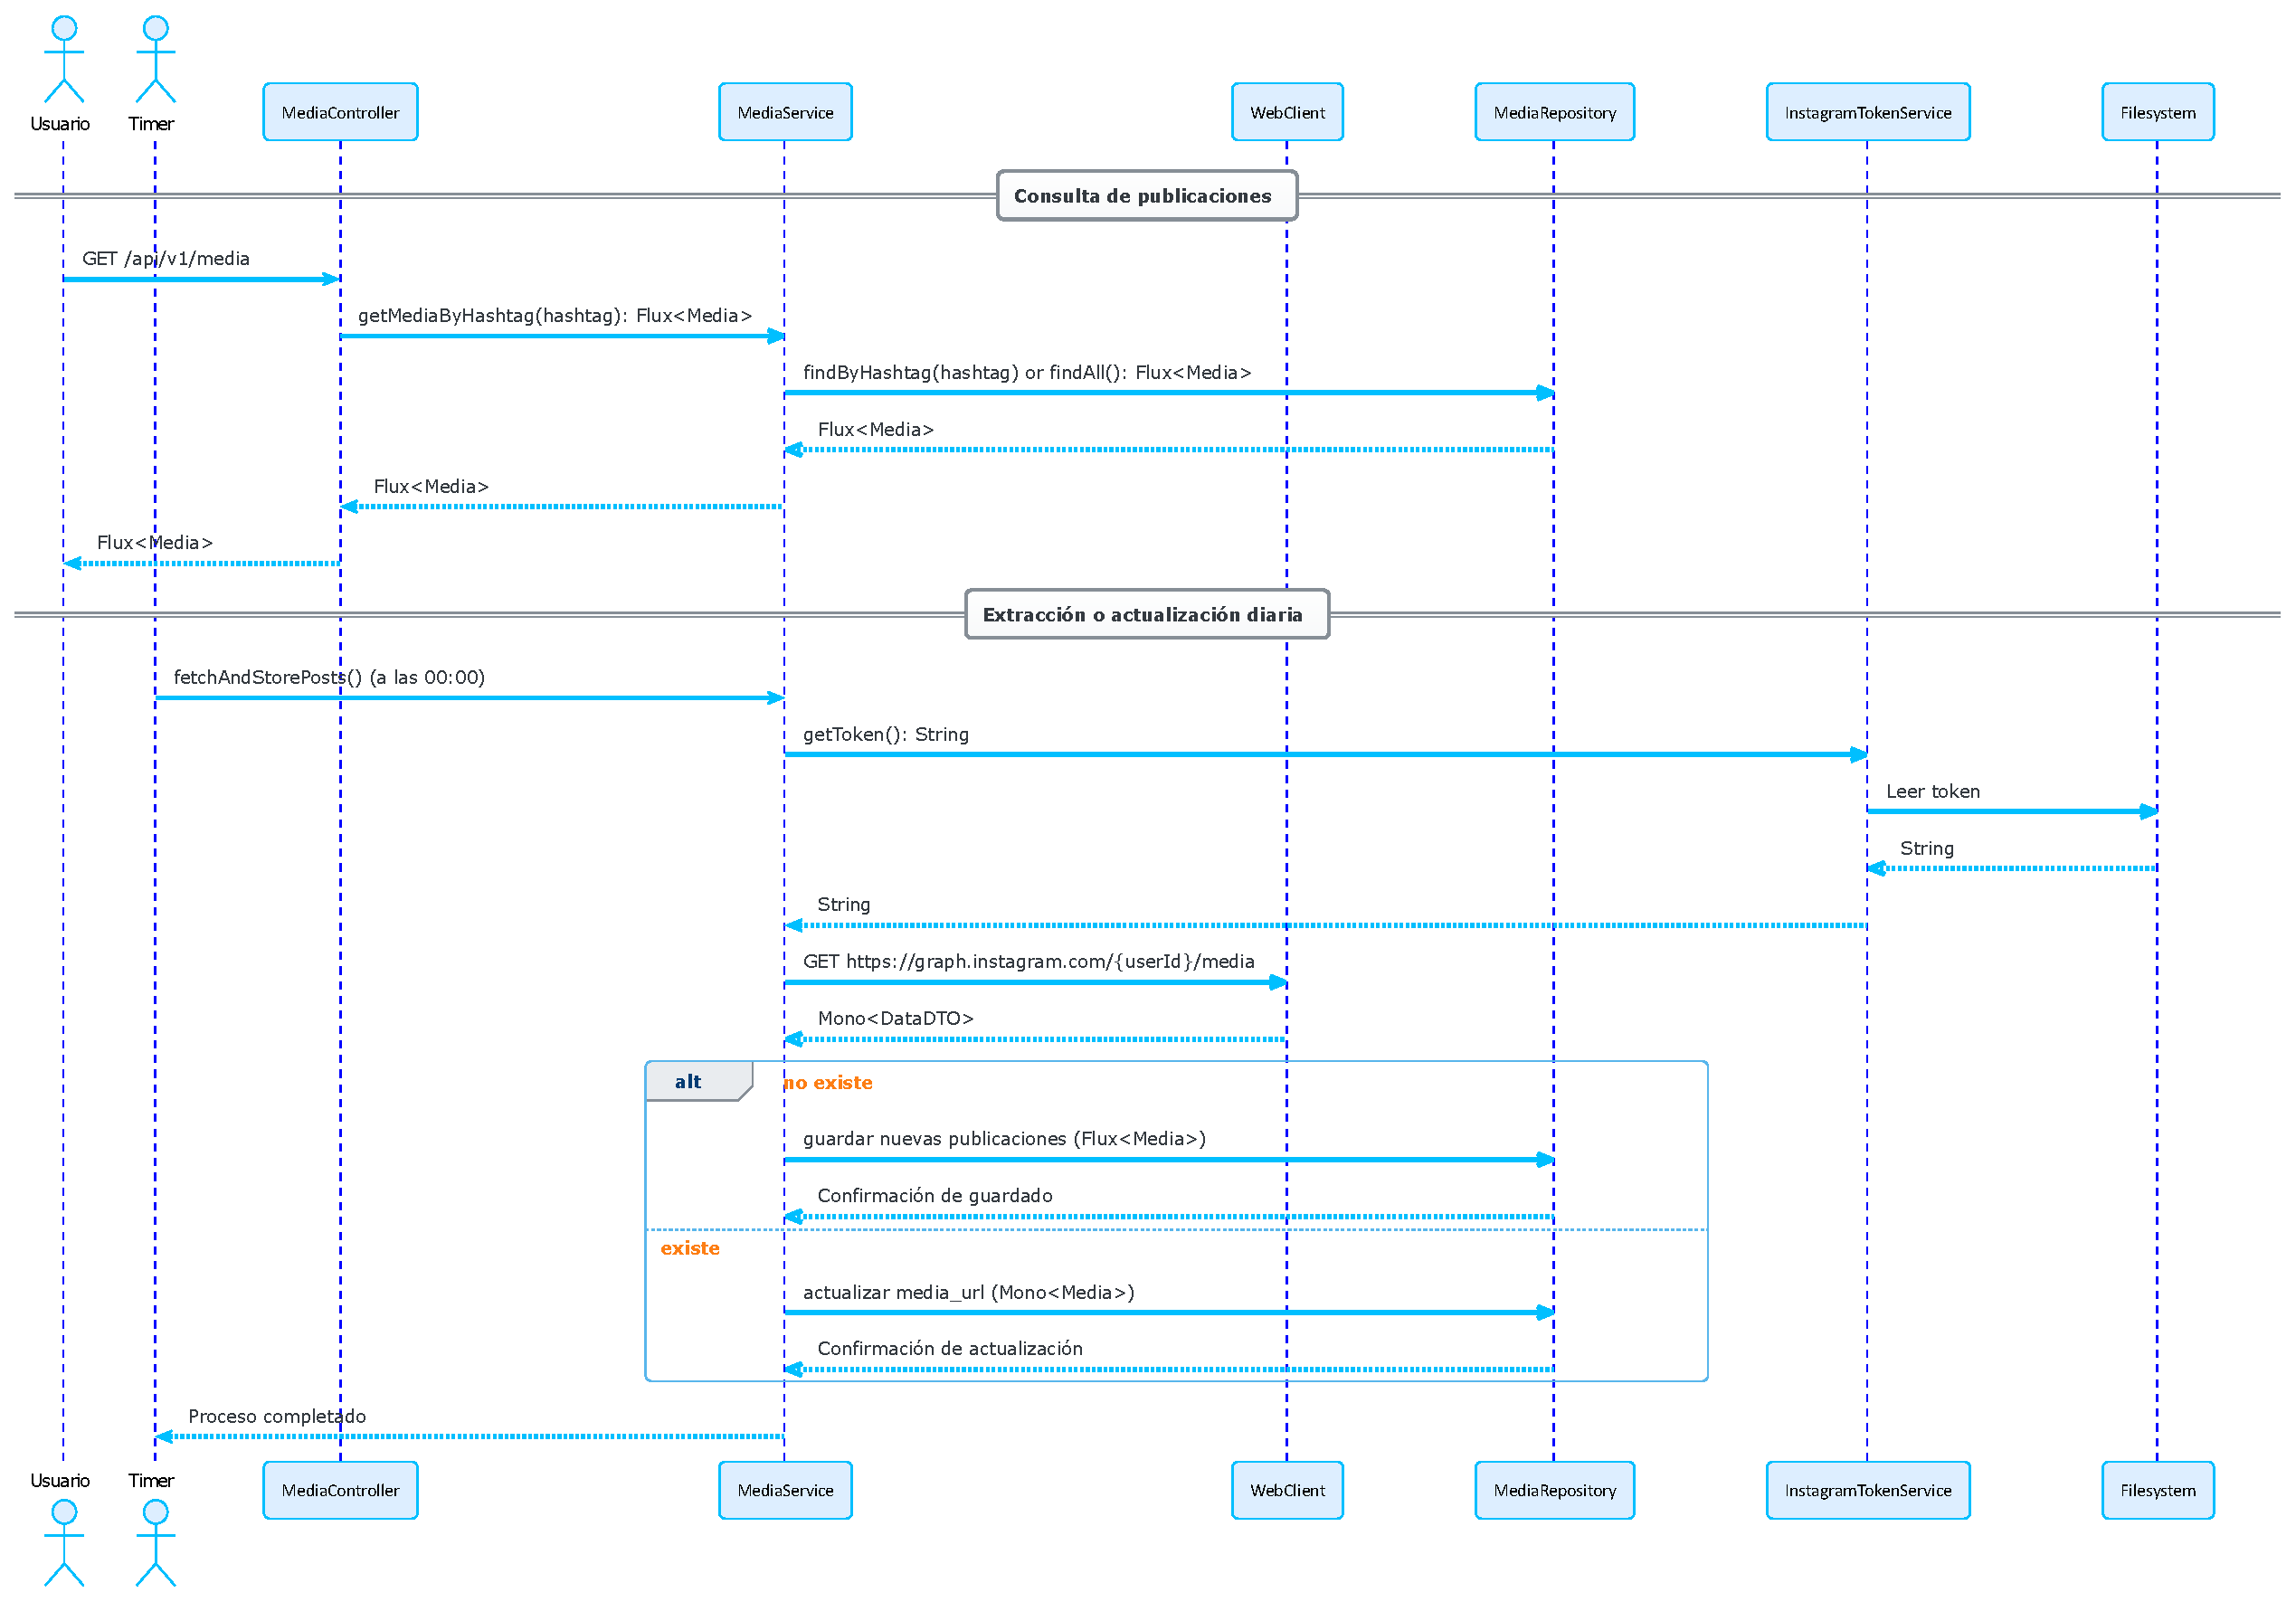
\includegraphics[width=1\textwidth]{figs/secuencia_publicaciones_baja.pdf}
    \caption{Diagrama de secuencia de consulta, extracción y actualización de publicaciones desde la \gls{API} de Instagram.\label{fig:secuencia_publicaciones_consulta}}
\end{figure}

Por otro lado, la Figura~\ref{fig:secuencia_publicaciones_token} muestra el procedimiento automatizado de renovación del token de acceso, esencial para mantener la conexión con la \gls{API}. Cada 30 días, el \texttt{InstagramTokenService} accede al sistema de archivos (\texttt{Filesystem}) para leer el token actual y realiza una solicitud a la ruta \texttt{refresh\_access\_token}. Una vez recibido el nuevo token, lo guarda de nuevo en el sistema de archivos. Este proceso garantiza la operatividad continua del sistema sin necesidad de intervención manual.

\begin{figure}[h!tb]
    \centering
    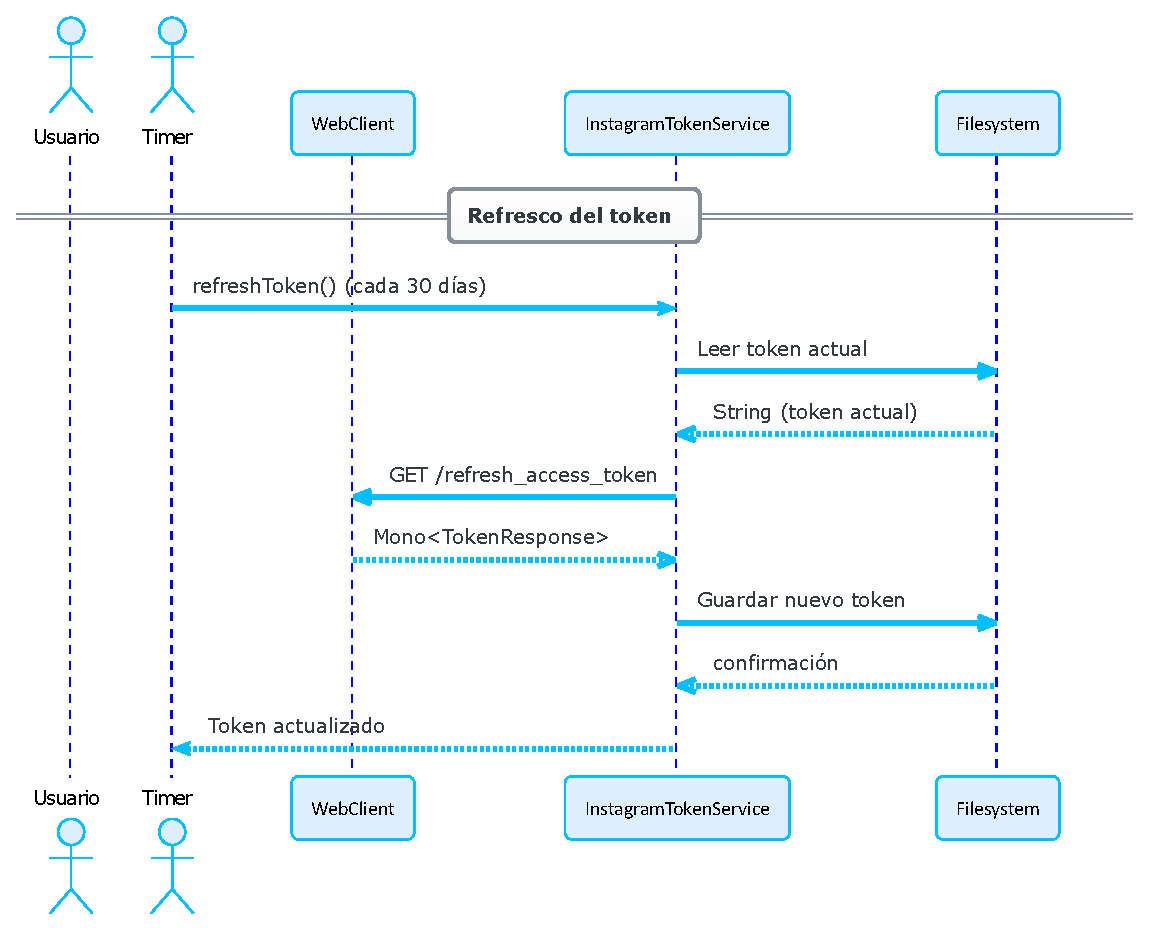
\includegraphics[width=1\textwidth]{figs/secuencia_publicaciones_token.pdf}
    \caption{Diagrama de secuencia del proceso de refresco del token de acceso (Subsistema de publicaciones).\label{fig:secuencia_publicaciones_token}}
\end{figure}


\section{Subsistema de previsión del tiempo}

En el subsistema de previsión del tiempo, el componente a especificar es el encargado de obtener información meteorológica de cara a la reserva del usuario. En la Figura~\ref{fig:secuencia_tiempo} se describe el proceso completo llevado a cabo cuando un usuario realiza una solicitud para consultar el pronóstico del tiempo en un rango de fechas determinado.

El flujo comienza cuando el \textbf{usuario} realiza una petición GET a \texttt{/api/v1/weather}, incluyendo dos parámetros de fecha. El \texttt{WeatherController} delega esta solicitud al \\ \texttt{WeatherService}, que realiza una iteración sobre cada fecha individual del rango indicado. Para cada una de estas fechas, primero intenta recuperar los datos desde la base de datos documental (\texttt{WeatherDataRepository}).

En caso de que los datos no se encuentren almacenados, el sistema evalúa si la fecha es histórica o si corresponde a una predicción futura. Si se trata de una fecha histórica (pasada o más allá de los próximos 15 días), se realiza una petición a la API de historial de Open Meteo. Si es una predicción (hasta 15 días en el futuro), se consulta la API de pronóstico. En ambos casos, la respuesta se procesa y se clasifica (por ejemplo: ``Lluvioso'', ``Frío'', ``Caluroso''...), y los datos resultantes se guardan en el repositorio para su reutilización futura.

Finalmente, el servicio devuelve todos los resultados al controlador, que responde al usuario con la lista de datos meteorológicos correspondiente.

\begin{figure}[h!tb]
    \centering
    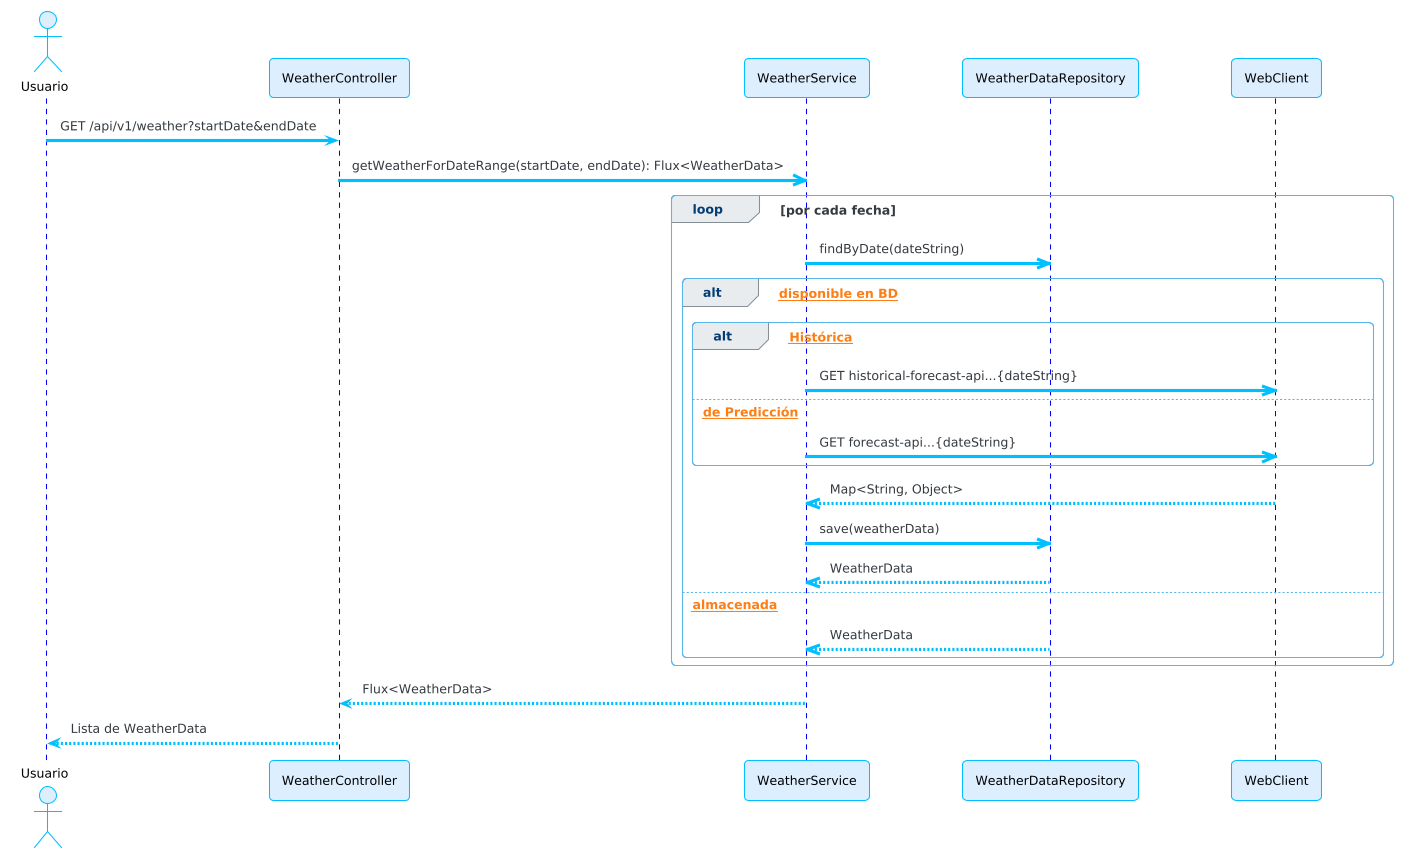
\includegraphics[width=1\textwidth]{figs/secuencia_tiempo.png}
    \caption{Diagrama de secuencia del componente de obtención de previsión del tiempo (Subsistema de previsión del tiempo).\label{fig:secuencia_tiempo}}
\end{figure}


\section{Diagrama de clases}
\label{ch:clases}
La Figura~\ref{fig:clases_disenyo} presenta el diagrama de clases que describe las principales entidades de un sistema de gestión de usuarios, reservas, opiniones y recursos. Este diagrama es fundamental para la comprensión de cómo interactúan las diferentes clases en el sistema.

\begin{sidewaysfigure}
    \centering
    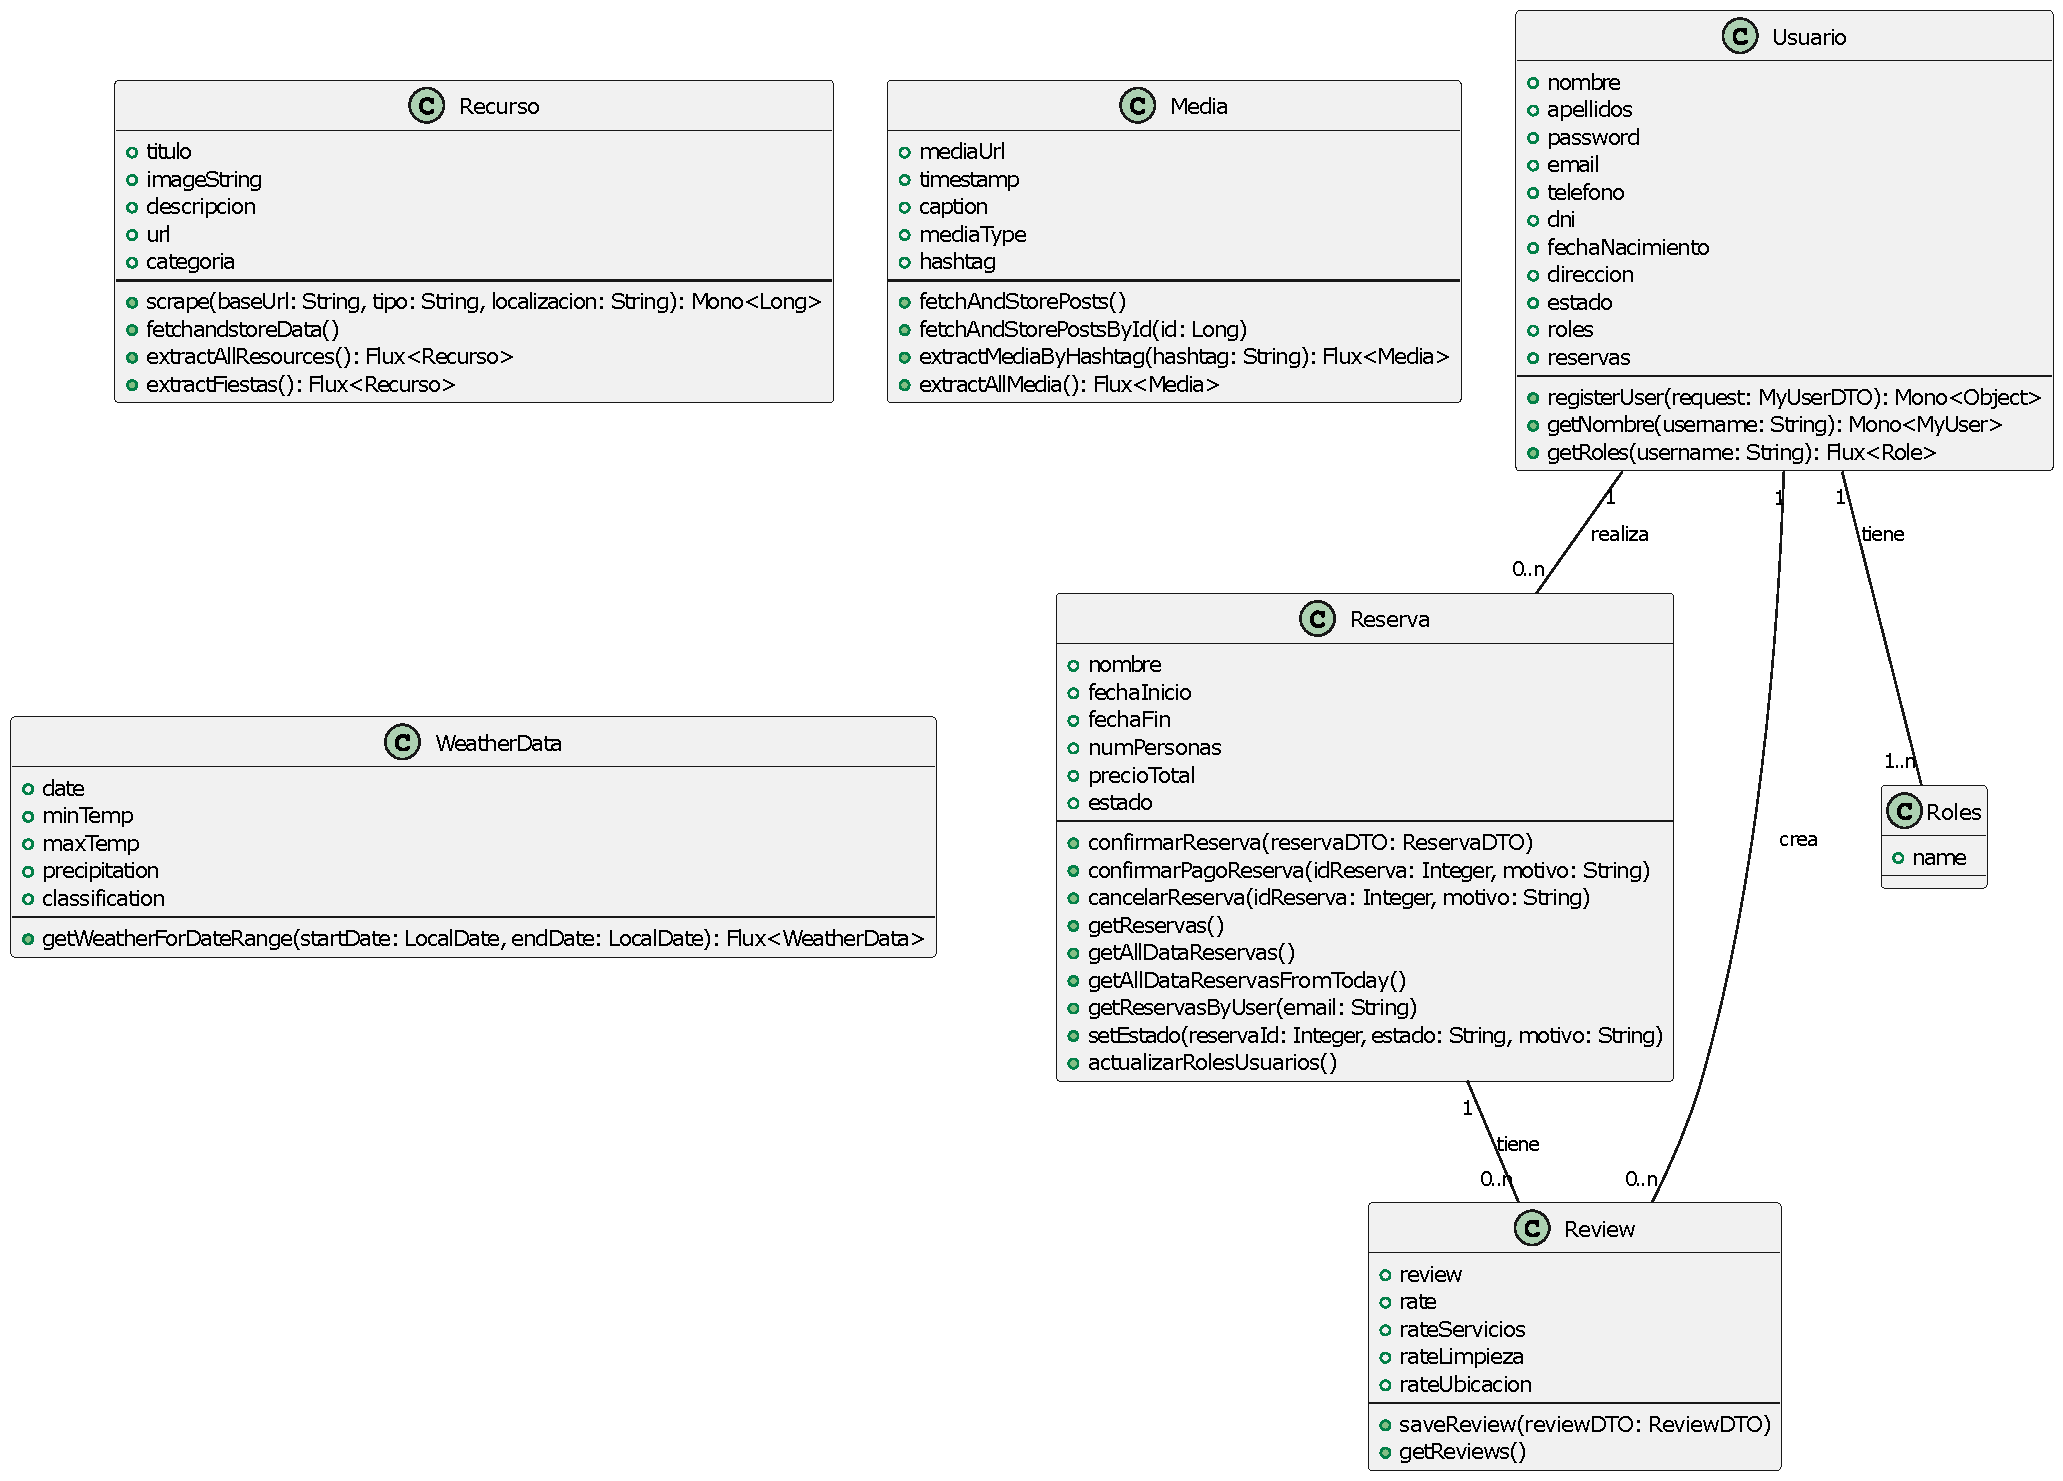
\includegraphics[width=0.8\textwidth]{figs/clases.pdf} 
    \caption{Diagrama de clases completo del sistema\label{fig:clases_disenyo}}
\end{sidewaysfigure}



Este diagrama muestra la estructura y relaciones entre las clases principales del sistema. La clase \texttt{Usuario} contiene atributos como nombre, apellidos, email, teléfono, entre otros. Esta clase también tiene métodos relacionados con el registro y obtención de usuarios y roles. La clase \texttt{Reserva} se encarga de la gestión de reservas, incluyendo la confirmación, cancelación y obtención de datos relacionados con las mismas. La clase \texttt{Review} gestiona las opiniones de los usuarios sobre los servicios, permitiendo registrar y obtener reseñas. Además, la clase \texttt{Recurso} gestiona los recursos de tipo información, como eventos y actividades, con métodos para obtener datos mediante scraping. La clase \texttt{Media} se encarga de manejar la información multimedia, como fotos y publicaciones en redes sociales, y la clase \texttt{WeatherData} almacena información relacionada con el clima, que puede ser consultada por rango de fechas.

Las relaciones entre las clases están representadas con las líneas de asociación. Por ejemplo, un \texttt{Usuario} puede tener múltiples \texttt{Reservas} y \texttt{Reviews}, mientras que una \texttt{Reserva} puede tener varias \texttt{Reviews}. Además, cada \texttt{Usuario} tiene uno o más \texttt{Roles}, los cuales determinan sus permisos dentro del sistema.

\section{Modelo de datos}

En cuanto a modelos de datos físicos se han definido tres modelos de datos para determinar las colecciones a generar en \texttt{MongoDB} y uno para las tablas relacionales en \texttt{PostgreSQL}. 

\subsection{Modelo físico de la base de datos relacional (\texttt{PostgreSQL})}

La Figura~\ref{fig:modelo_datos_postgres} muestra el modelo físico de datos de la base de datos relacional, implementado en \texttt{PostgreSQL}. El diagrama entidad-relación describe la estructura de las tablas, los campos principales y las relaciones de integridad referencial existentes en el sistema.

\begin{figure}[h!tb]
\centering
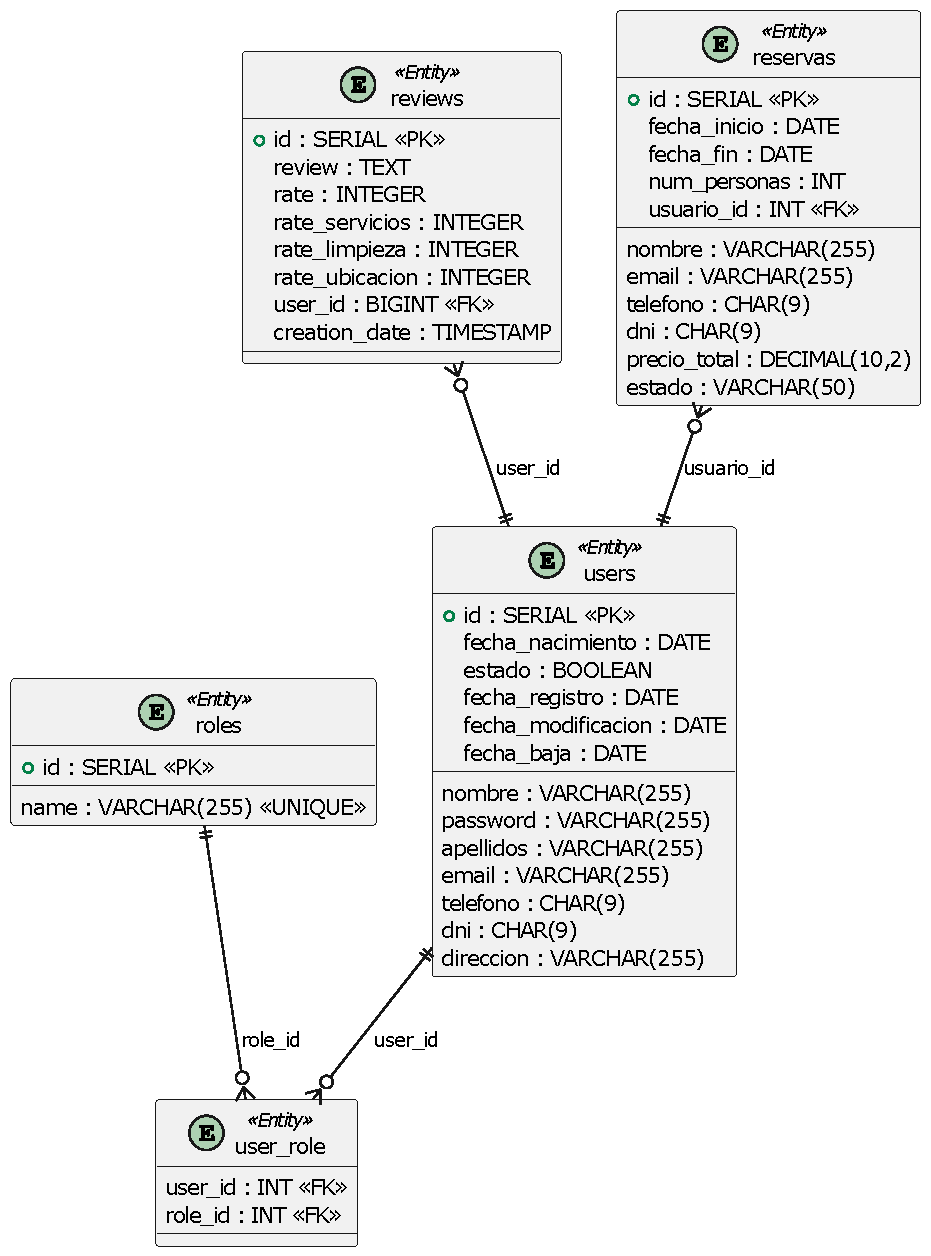
\includegraphics[width=0.6\textwidth]{figs/pg_sifico.pdf}
\caption{Modelo físico de la base de datos relacional \texttt{PostgreSQL}.\label{fig:modelo_datos_postgres}}
\end{figure}

El modelo se compone de las siguientes tablas:

\texttt{users}: Contiene los datos de los usuarios del sistema. Incluye campos como \texttt{id} (clave primaria, tipo \texttt{SERIAL}), \texttt{fecha\_nacimiento}, \texttt{estado}, \texttt{fecha\_registro}, \texttt{fecha\_modificacion}, \texttt{fecha\_baja}, \texttt{nombre}, \texttt{password}, \texttt{apellidos}, \texttt{email}, \texttt{telefono}, \texttt{dni} y \texttt{direccion}.\\
Nota: El campo \texttt{password} se almacena cifrado tanto a nivel de base de datos como a nivel de aplicación, siguiendo buenas prácticas de seguridad y protección de la información sensible de los usuarios. Esta tabla se encuentra referenciada por otras entidades.

\texttt{roles}: Define los posibles roles de usuario en el sistema. Está formada por el campo \texttt{id} (clave primaria, tipo \texttt{SERIAL}) y \texttt{name} (tipo \texttt{VARCHAR}, único).

\texttt{user\_role}: Tabla intermedia que implementa la relación muchos-a-muchos entre usuarios y roles. Incluye los campos \texttt{user\_id} y \texttt{role\_id}, ambos claves foráneas que referencian a las tablas \texttt{users} y \texttt{roles}, respectivamente.

\texttt{reviews}: Almacena las valoraciones de los usuarios. Incluye \texttt{id} (clave primaria), \texttt{review} (texto), \texttt{rate}, \texttt{rate\_servicios}, \texttt{rate\_limpieza}, \texttt{rate\_ubicacion} (todos de tipo \texttt{INTEGER}), \texttt{user\_id} (clave foránea a \texttt{users}) y \texttt{creation\_date} (timestamp).

\texttt{reservas}: Recoge la información de las reservas realizadas. Sus campos principales son \texttt{id} (clave primaria), \texttt{fecha\_inicio}, \texttt{fecha\_fin}, \texttt{num\_personas}, \texttt{usuario\_id} (clave foránea a \texttt{users}), \texttt{nombre}, \texttt{email}, \texttt{telefono}, \texttt{dni}, \texttt{precio\_total} y \texttt{estado}.

El diagrama incluye las relaciones de integridad referencial entre las tablas mediante claves foráneas (\texttt{user\_id}, \texttt{role\_id} y \texttt{usuario\_id}), asegurando la consistencia de los datos a través de las asociaciones indicadas.

\subsection{Modelo de datos de la base de datos no relacional \texttt{MongoDB}}

La Figura~\ref{fig:modelo_datos_mongodb} muestra el modelo físico de datos correspondiente a las colecciones de la base de datos \texttt{MongoDB} utilizadas en el sistema. El diagrama representa tres colecciones principales: \texttt{recursos}, \texttt{media} y \texttt{weather\_data}, cada una con su respectiva estructura de campos.

\begin{figure}[h!tb]
\centering
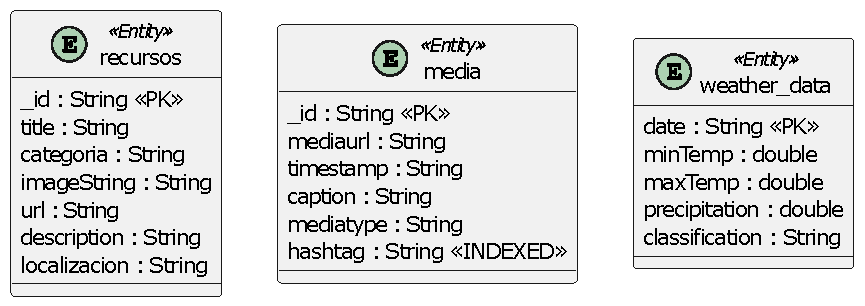
\includegraphics[width=0.6\textwidth]{figs/mongo_fisico.pdf}
\caption{Modelo físico de la base de datos no relacional \texttt{MongoDB}.\label{fig:modelo_datos_mongodb}}
\end{figure}


\texttt{recursos}: Esta colección contiene documentos identificados por el campo \texttt{\_id} (clave primaria), y almacena los siguientes atributos: \texttt{title}, \texttt{categoria}, \texttt{imageString}, \texttt{url}, \texttt{description} y \texttt{localizacion}, todos de tipo \texttt{String}.

\texttt{media}: Los documentos de la colección \texttt{media} disponen de los campos \texttt{\_id} (clave primaria), \texttt{mediaurl}, \texttt{timestamp}, \texttt{caption}, \texttt{mediatype} y \texttt{hashtag}, todos de tipo \texttt{String}. El campo \texttt{hashtag} está indexado, ya que en el desarrollo se van a realizar la mayoría de búsquedas a través de él, por lo que al indexarlo mejorará la velocidad en la búsqueda de documentos.

\texttt{weather\_data}: Cada documento en esta colección se identifica por el campo \texttt{date} (clave primaria, de tipo \texttt{String}), y contiene los campos \texttt{minTemp}, \texttt{maxTemp}, \texttt{precipitation} (de tipo \texttt{double}) y \texttt{classification} (de tipo \texttt{String}).

En el modelo presentado no existen relaciones explícitas entre colecciones, ya que MongoDB utiliza un enfoque orientado a documentos donde cada colección es independiente y puede escalar de manera autónoma. Los tipos de datos y claves principales están reflejados en el propio diagrama.

\section{Despliegue del sistema}\label{ch:despliegue}

El presente sistema está diseñado para ejecutarse sobre una arquitectura de contenedores orquestada con \gls{kubernetes}, de forma que pueda desplegarse en cualquier proveedor de servicios en la nube. 
En este apartado se detalla la infraestructura de despliegue propuesta, representada visualmente en la Figura~\ref{fig:diagrama_despliegue} mediante un diagrama de despliegue, que resume gráficamente la organización de los servicios, contenedores, volúmenes persistentes y conexiones internas en el clúster de Kubernetes.

\begin{sidewaysfigure}
    \centering
    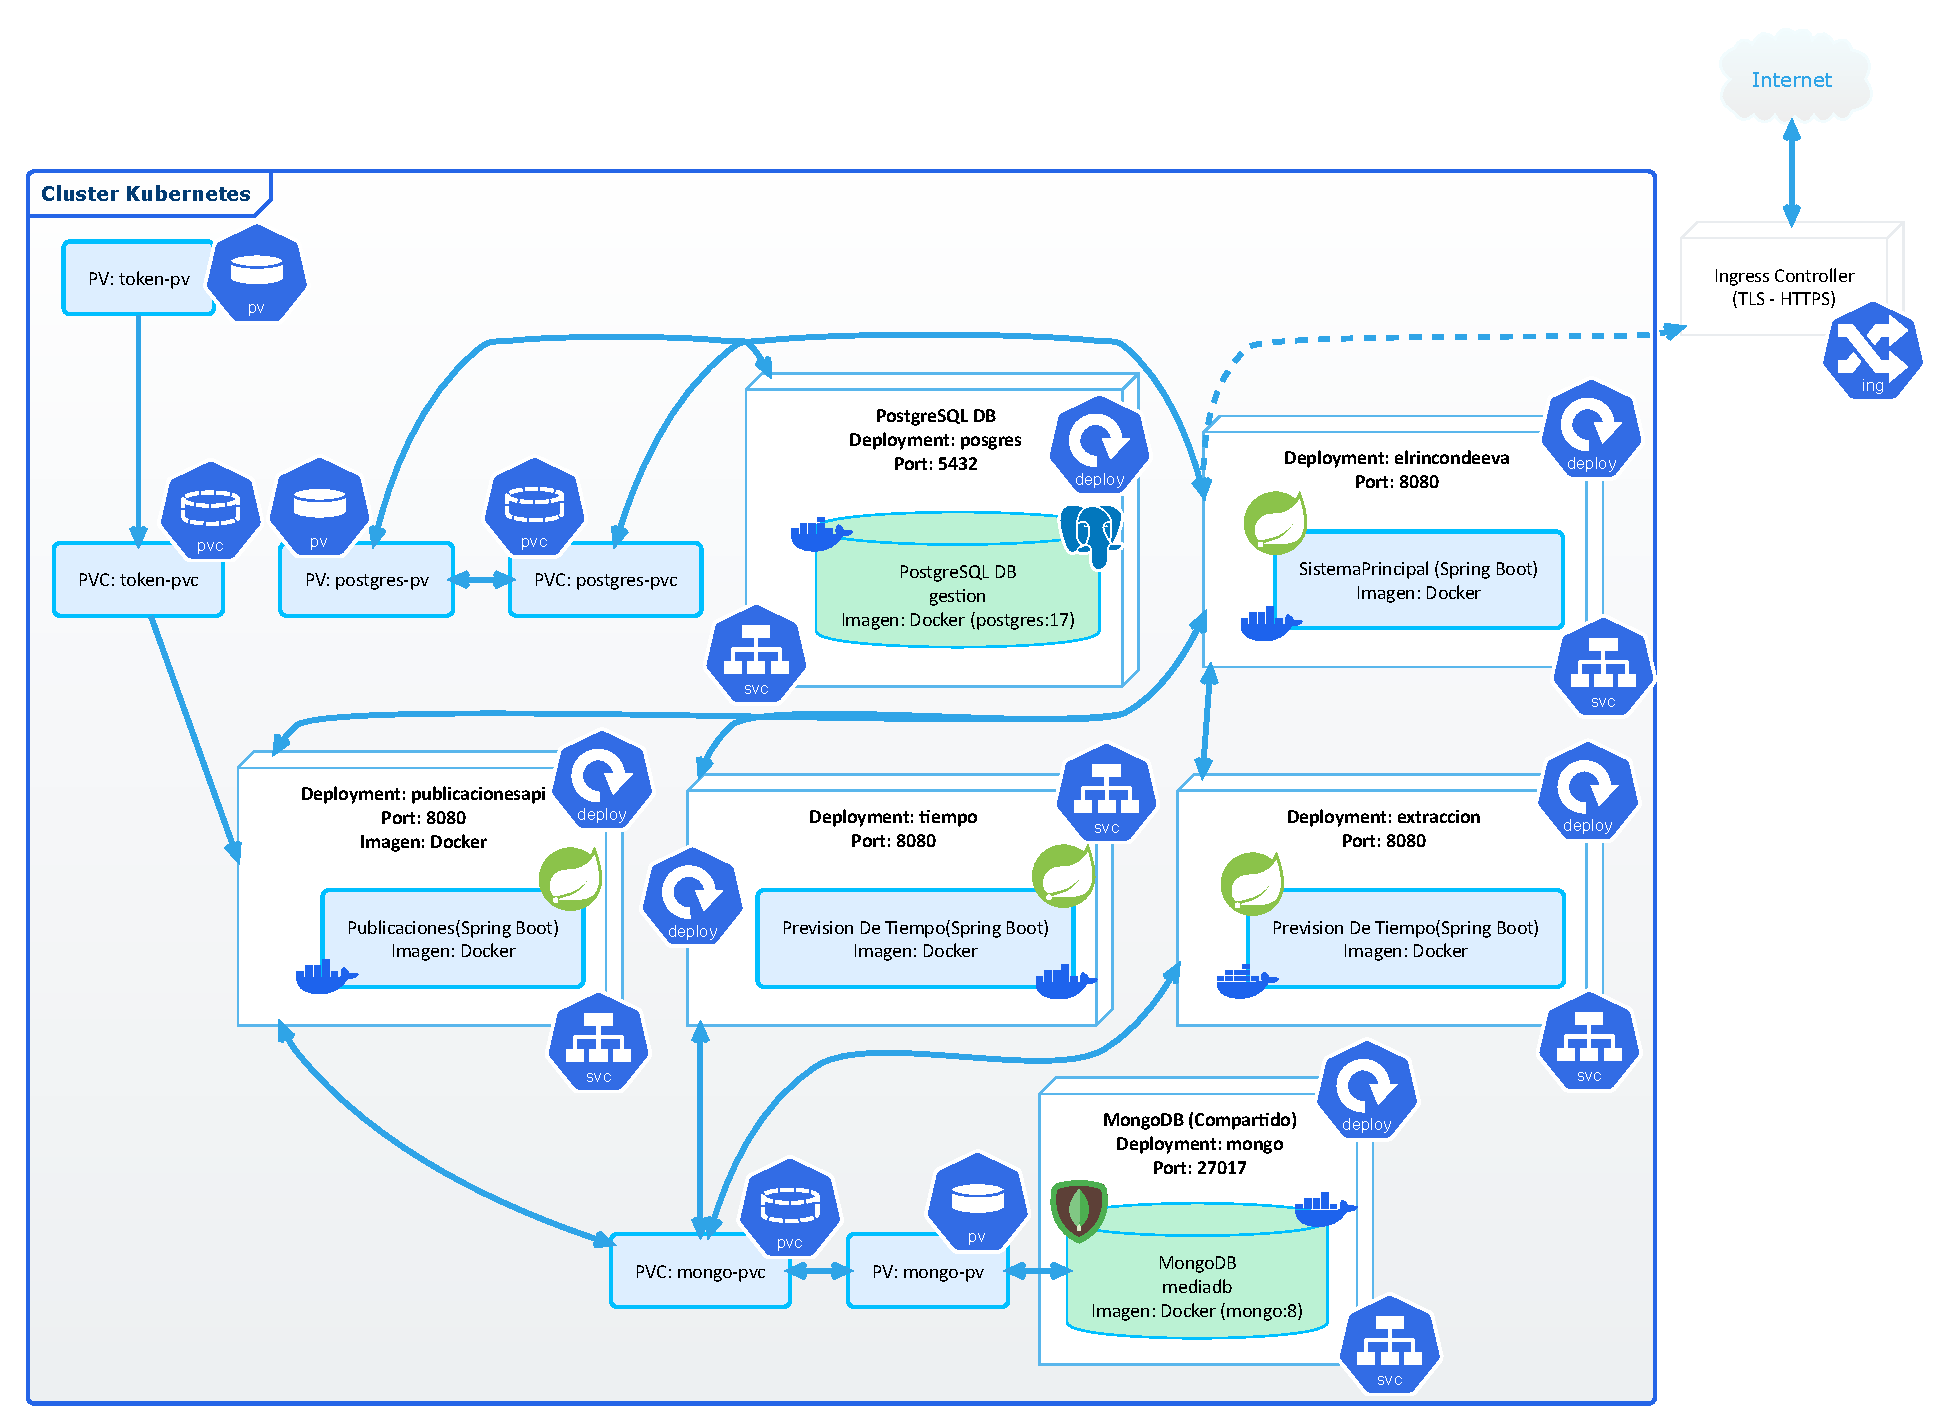
\includegraphics[width=0.8\textwidth]{figs/despliegue-nube.pdf}
    \caption{Diagrama de despliegue del sistema basado en contenedores Docker sobre arquitectura Kubernetes.\label{fig:diagrama_despliegue}}
\end{sidewaysfigure}

El sistema se compone de una aplicación principal, encapsulada en un contenedor Docker bajo el nombre de \texttt{elrincondeeva}, desplegada como un \texttt{Deployment} en Kubernetes. Esta aplicación central es responsable de coordinar la lógica de negocio y canalizar las peticiones hacia los distintos \glspl{microservicio} del sistema: \texttt{Publicaciones}, \texttt{PrevisionDeTiempo} y \texttt{RecursosWeb}, también empaquetados como contenedores Docker y desplegados como pods independientes dentro del clúster.

La comunicación externa con el sistema se realiza a través de un \gls{ingress} que expone el servicio principal mediante protocolo \gls{https}. Este \texttt{Ingress Controller} actúa como único punto de entrada al sistema, redirigiendo las peticiones entrantes al contenedor correspondiente del servicio principal, aunque se mantiene la flexibilidad para exponer directamente otros servicios si fuera necesario en un futuro.

En cuanto al almacenamiento persistente, el sistema utiliza dos bases de datos. Por un lado, una instancia de \gls{postgresql} para la gestión de datos relacionales, asociada exclusivamente al contenedor principal. Esta base de datos se monta sobre un volumen persistente (\gls{pv}) y un reclamo (\gls{pvc}) propio, garantizando la durabilidad de los datos. Por otro lado, los microservicios de \texttt{Publicaciones}, \texttt{PrevisionDeTiempo} y \texttt{RecursosWeb} comparten una base de datos \gls{mongodb} desplegada como un único contenedor y montada igualmente sobre su propio par \texttt{PV}/\texttt{PVC}.

Una particularidad del microservicio \texttt{Publicaciones} es que requiere almacenar de forma persistente un \gls{token} de acceso para consultar la \gls{API} de Instagram. Para ello, se ha montado un volumen persistente específico (\texttt{token-pv}) a través de un \texttt{PVC}, que permite mantener dicho archivo de manera duradera. Esta solución evita el uso de \texttt{Secrets} o \texttt{ConfigMaps}, que no serían adecuados debido a la necesidad de escritura dinámica sobre el archivo.

\section{Despliegue en entorno local}

Durante la fase de desarrollo, se ha optado por un despliegue en entorno local que permite una ejecución sencilla de cada uno de los componentes del sistema sin depender de herramientas de orquestación como \gls{kubernetes} ni de contenedores \gls{docker}. En este modelo, cada microservicio se ejecuta como una aplicación independiente en la misma máquina o red local, y se comunican entre sí mediante llamadas HTTP directas a través de diferentes puertos.

La Figura~\ref{fig:diagrama_despliegue_local} muestra el diagrama de despliegue utilizado durante el desarrollo local. En este esquema, cada componente desarrollado con \gls{springboot} (\texttt{SistemaPrincipal}, \texttt{Publicaciones}, \texttt{PrevisionDeTiempo} y \texttt{RecursosWeb}) se ejecuta como una aplicación independiente, expuesta a través de su propio puerto. Asimismo, las bases de datos \gls{postgresql} y \gls{mongodb} se ejecutan como servicios locales tradicionales.

A diferencia de la arquitectura en la nube descrita anteriormente, donde las comunicaciones están encapsuladas y controladas mediante un \gls{ingress}, en el entorno local cada servicio es accesible desde el exterior a través de \texttt{localhost} y su respectivo puerto. Esto implica que cualquier consumidor que conozca el puerto puede acceder directamente a cualquiera de los servicios, lo cual reduce el aislamiento y la seguridad del sistema. En el modelo de nube, sin embargo, solo se permite el acceso desde Internet al servicio principal (\texttt{SistemaPrincipal}) gracias al uso del \gls{ingress} y protocolos seguros como \gls{https}.

Este enfoque local permite realizar pruebas y desarrollos de manera más rápida y sin necesidad de infraestructura adicional, aunque se recomienda restringir su uso a entornos controlados, dado que carece de mecanismos de seguridad avanzados.

\begin{figure}[h!tb]
    \centering
    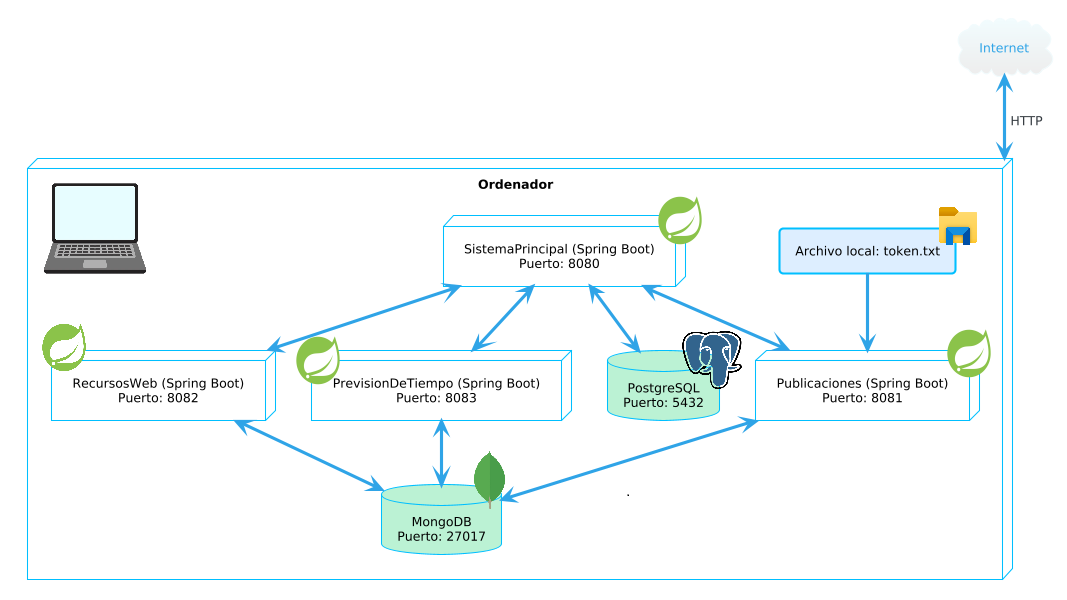
\includegraphics[width=\textwidth]{figs/despliegue_local.png}
    \caption{Diagrama de despliegue del sistema en entorno local.\label{fig:diagrama_despliegue_local}}
\end{figure}
